\documentclass[sunil1,ChapterTOCs]{sunil}
\usepackage[utf8]{inputenc}
\usepackage{amssymb}
\usepackage{amsmath}
\usepackage{graphicx}
\usepackage{subfigure}
%\usepackage{epsfig}
\usepackage{makeidx}
\usepackage{listings}
\usepackage{caption}
\usepackage{courier}
\usepackage{color}
\usepackage[sectionbib]{bibunits}
\usepackage{multicol}
\usepackage{alltt}


\frenchspacing
\tolerance=5000

\include{Chapters/chapter1/preamble}

\makeatletter


\makeatother

\newtheorem{proposition}{Proposition}
\newtheorem{proof}{Proof}




 \lstset{
         basicstyle=\footnotesize\ttfamily, % Standardschrift
         %numbers=left,               % Ort der Zeilennummern
         numberstyle=\tiny,          % Stil der Zeilennummern
         %stepnumber=2,               % Abstand zwischen den Zeilennummern
         numbersep=5pt,              % Abstand der Nummern zum Text
         tabsize=2,                  % Groesse von Tabs
         extendedchars=true,         %
         breaklines=true,            % Zeilen werden Umgebrochen
         keywordstyle=\color{red},
    		frame=b,         
 %        keywordstyle=[1]\textbf,    % Stil der Keywords
 %        keywordstyle=[2]\textbf,    %
 %        keywordstyle=[3]\textbf,    %
 %        keywordstyle=[4]\textbf,   \sqrt{\sqrt{}} %
         stringstyle=\color{white}\ttfamily, % Farbe der String
         showspaces=false,           % Leerzeichen anzeigen ?
         showtabs=false,             % Tabs anzeigen ?
         xleftmargin=17pt,
         framexleftmargin=17pt,
         framexrightmargin=5pt,
         framexbottommargin=4pt,
         %backgroundcolor=\color{lightgray},
         showstringspaces=false      % Leerzeichen in Strings anzeigen ?        
 }
 \lstloadlanguages{% Check Dokumentation for further languages ...
         %[Visual]Basic
         %Pascal
         C
         %C++
         %XML
         %HTML
         %Java
 }
  %\DeclareCaptionFont{blue}{\color{blue}} 

  %\captionsetup[lstlisting]{singlelinecheck=false, labelfont={blue}, textfont={blue}}
\DeclareCaptionFont{white}{\color{white}}
\DeclareCaptionFormat{listing}{\colorbox[cmyk]{0.43, 0.35, 0.35,0.01}{\parbox{\textwidth}{\hspace{15pt}#1#2#3}}}
\captionsetup[lstlisting]{format=listing,labelfont=white,textfont=white, singlelinecheck=false, margin=0pt, font={bf,footnotesize}}



\makeindex

\begin{document}


%%bibliography style to adopt
\bibliographyunit[\chapter]
\defaultbibliographystyle{plain}



\title{Designing Scientific Applications on GPUs }

\author{Raphaël Couturier}

\maketitle

\frontmatter
\chapter*{Foreward}
I am delighted to introduce the first book on Multimedia Data Mining.  When I came to know about this book project undertaken by two of the most active young researchers in the field, I was pleased that this book is coming in early stage of a field that will need it more than most fields do.  In most emerging research fields, a book can play a significant role in bringing some maturity to the field.  Research fields advance through research papers.  In research papers, however, only a limited perspective could be provided about the field, its application potential, and the techniques required and already developed in the field.  A book gives such a chance.  I liked the idea that there will be a book that will try to unify the field by bringing in disparate topics already available in several papers that are not easy to find and understand.  I was supportive of this book project even before I had seen any material on it.  The project was a brilliant and a bold idea by two active researchers.  Now that I have it on my screen, it appears to be even a better idea.  

Multimedia started gaining recognition in 1990s as a field.  Processing, storage, communication, and capture and display technologies had advanced enough that researchers and technologists started building approaches to combine information in multiple types of signals such as audio, images, video, and  text.  Multimedia computing and communication techniques recognize correlated information in multiple sources as well as insufficiency of information in any individual source.    By properly selecting sources to provide complementary information, such systems aspire, much like human perception system, to create a holistic picture of a situation using only partial information from separate sources.

Data mining is a direct outgrowth of progress in data storage and processing speeds.  When it became possible to store large volume of data and run different statistical computations to explore all possible and even unlikely correlations among data, the field of data mining was born.  Data mining allowed people to hypothesize relationships among data entities and explore support for those.  This field has been put to applications in many diverse domains and keeps getting more applications.  In fact many new fields are direct outgrowth of data mining and it is likely to become a powerful computational tool.\vadjust{\vfill\pagebreak}

\thispagestyle{empty}


\include{frontmatter/preface}

\listoffigures
\listoftables
\tableofcontents

\mainmatter

\include{Chapters/symbollist}

\setcounter{page}{1}
\part{This is a Part}
%\chapterauthor{Raphaël Couturier}{Femto-ST Institute, University of Franche-Comte}


\chapter{Presentation of the GPU architecture and of the Cuda environment}
\label{chapter1}

\section{Introduction}\label{ch1:intro}

This chapter introduces the Graphics  Processing Unit (GPU) architecture and all
the concepts needed to understand how GPUs  work and can be used to speed up the
execution of some algorithms. First of all this chapter gives a brief history of
the development  of Graphics  card until they  have been  used in order  to make
general   purpose   computation.    Then   the   architecture  of   a   GPU   is
illustrated.  There  are  many  fundamental  differences between  a  GPU  and  a
tradition  processor. In  order  to benefit  from the  power  of a  GPU, a  Cuda
programmer needs to use threads. They have some particularities which enable the
Cuda model to be efficient and scalable when some constraints are addressed.



\section{Brief history of Video Card}

Video  cards or Graphics  cards have  been introduced  in personal  computers to
produce  high quality graphics  faster than  classical Central  Processing Units
(CPU) and  to alleviate CPU from this  task. In general, display  tasks are very
repetitive and very specific.  Hence,  some manufacturers have produced more and
more sophisticated video cards, providing 2D accelerations then 3D accelerations,
then some  light transforms. Video cards  own their own memory  to perform their
computation.  For at least two decades, every personal computer has had a video
card which is simple for  desktop computers or which provides many accelerations
for game and/or  graphic oriented computers.  In the  latter case, graphic cards
may be more expensive than a CPU.

Since  2000, video  cards have  allowed  users to  apply arithmetic  operations
simultaneously on a sequence of  pixels, also later called stream processing. In
this case, the information of the pixels (color, location and other information) are
combined in order  to produce a pixel  color that can be displayed  on a screen.
Simultaneous  computations are  provided  by shaders  which calculate  rendering
effects on  graphics hardware with a  high degree of  flexibility. These shaders
handles the stream data with pipelines.


Some researchers  tried to  apply those operations  on other  data, representing
something different  from pixels,  and consequently this  resulted in  the first
uses of video cards for  performing general purpose computation. The programming
model  was not  easy  to use  at  all and  was very  dependent  of the  hardware
constraints.   More precisely  it consisted  in using  either DirectX  of OpenGL
functions  providing  an  interface  to  some classical  operations  for  videos
operations  (memory  transfers,  texture  manipulation,  ...).   Floating  point
operations were  most of the  time unimaginable.  Obviously when  something went
wrong, programmers had no way (and neither the tools) to detect it.

\section{GPGPU}

In order  to benefit from the computing  power of more recent  video cards, Cuda
was first proposed in 2007 by  NVidia. It unifies the programming model for some
of  their most performant  video cards.   Cuda~\cite{ch1:cuda} has  quickly been
considered by  the scientific community as  a great advance  for general purpose
graphics processing unit (GPGPU)  computing.  Of course other programming models
have been  proposed. The  other well-known alternative  is OpenCL which  aims at
proposing an alternative to Cuda  and which is multi-platform and portable. This
is a  great advantage since  it is even  possible to execute OpenCL  programs on
traditional CPUs.  The main drawback is that it is less tight with the hardware
and  consequently sometimes  provides  less efficient  programs. Moreover,  Cuda
benefits from  more mature compilation and optimization  procedures.  Other less
known environments  have been proposed, but  most of them have  been stopped, for
example  we can  cite: FireStream  by ATI  which is  not maintained  anymore and
replaced by  OpenCL, BrookGPU by  Standford University~\cite{ch1:Buck:2004:BGS}.
Another environment based  on pragma (insertion of pragma  directives inside the
code to  help the compiler to generate  efficient code) is call  OpenACC.  For a
comparison with OpenCL, interested readers may refer to~\cite{ch1:CMR:12}.



\section{Architecture of current GPUs}

The architecture  \index{architecture of  a GPU} of  current GPUs  is constantly
evolving.  Nevertheless  some trends remain constant  throughout this evolution.
Processing units composing a GPU are  far more simple than a traditional CPU but
it is much easier to integrate many computing units inside a GPU card than to do
so with many cores inside a CPU. This is due to the fact that the cores of a GPU are
simpler than the cores of a CPU.  In  2012, the most powerful GPUs own more than 500
cores       and       the       most       powerful      CPUs       have       8
cores. Figure~\ref{ch1:fig:comparison_cpu_gpu} shows  the number of cores inside
a  CPU  and  inside a  GPU.   In  fact,  in  a  current NVidia  GPU,  there  are
multiprocessors which have 32 cores (for example on Fermi cards). The core clock
of CPU is  generally around 3GHz and  the one of GPU is  about 1.5GHz.  Although
the core clock of GPU cores is slower, the amount of cores inside a GPU provides
more computational power.  This measure is commonly represented by the number of
floating point operation  per seconds. Nowadays the most powerful  GPUs provide more
than   1TFlops,  i.e.    $10^{12}$   floating  point   operations  per   second.
Nevertheless  GPUs are very  efficient to  perform some  operations but  not all
kinds of operations. They are very efficient to execute repetitive work in which
only  the data  change. It  is important  to keep  in mind  that multiprocessors
inside a GPU have 32 cores. Later we will see that these 32 cores need to do the
same work to get maximum performance.

\begin{figure}[b!]
\centerline{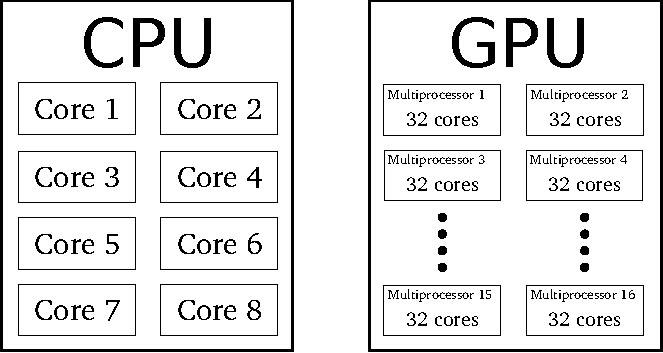
\includegraphics[]{Chapters/chapter1/figures/nb_cores_CPU_GPU.pdf}}
\caption{Comparison of number of cores in a CPU and in a GPU.}
%[Comparison of number of cores in a CPU and in a GPU]
\label{ch1:fig:comparison_cpu_gpu}
\end{figure}

On the most powerful  GPU cards, called Fermi, multiprocessors  are called streaming
multiprocessors  (SM). Each  SM contains  32  cores and  is able  to perform  32
floating points or integer operations on  32 bits numbers per clock or 16 floating
points  on  64 bits number  per  clock. SMs  have  their  own registers,  execution
pipelines and caches.  On Fermi architecture,  there are 64Kb shared memory + L1
cache  and 32,536 32bits  registers per  SM. More  precisely the  programmer can
decide what amount  of shared memory and  L1 cache SM can use.  The constraint is
that the sum of both amounts should be less or equal to 64Kb.

Threads are used to  benefit from the important number of cores  of a GPU. Those
threads    are   different    from    traditional   threads    for   CPU.     In
chapter~\ref{chapter2},  some  examples of  GPU  programming  will explicit  the
details of  the GPU  threads. However,  threads are gathered  into blocks  of 32
threads, called ``warps''. Those warps  are important when designing an algorithm
for GPU.


Another big  difference between CPU and GPU  is the latency of  memory.  In CPU,
everything is optimized  to obtain a low latency  architecture. This is possible
through  the  use  of  cache  memories. Moreover,  nowadays  CPUs  perform  many
performance optimizations  such as speculative execution  which roughly speaking
consists in executing  a small part of  code in advance even if  later this work
reveals itself  to be  useless. On the  contrary, GPUs  do not have  low latency
memory.   In comparison GPUs  have small  cache memories.  Nevertheless the
architecture of GPUs is optimized  for throughput computation and it takes into
account the memory latency.



\begin{figure}[b!]
\centerline{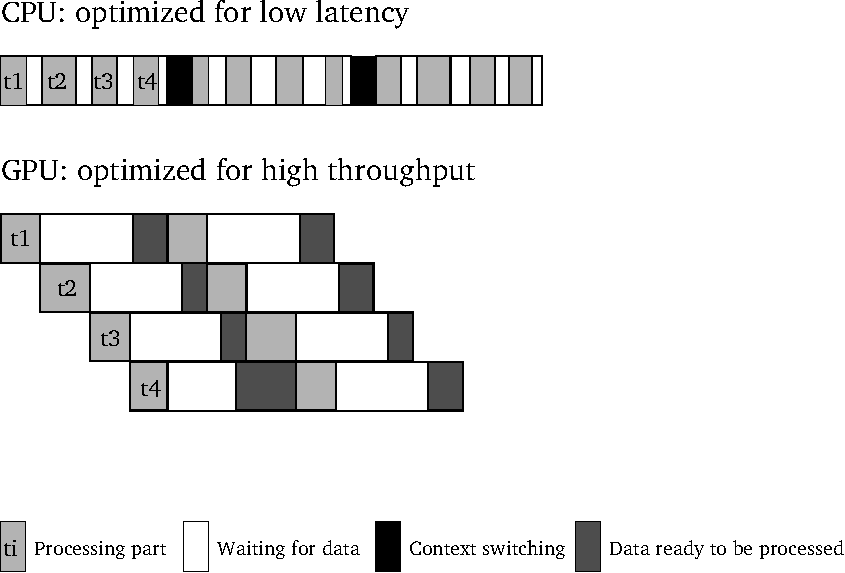
\includegraphics[scale=0.7]{Chapters/chapter1/figures/low_latency_vs_high_throughput.pdf}}
\caption{Comparison of low latency of CPU and high throughput of GPU.}
\label{ch1:fig:latency_throughput}
\end{figure}

Figure~\ref{ch1:fig:latency_throughput}  illustrates   the  main  difference  of
memory latency between a CPU and a  GPU. In a CPU, tasks ``ti'' are executed one
by one with a short memory latency to get the data to process. After some tasks,
there is  a context switch  that allows the  CPU to run  concurrent applications
and/or multi-threaded  applications. Memory latencies  are longer in a  GPU, the
the  principle  to   obtain  a  high  throughput  is  to   have  many  tasks  to
compute. Later we  will see that those tasks are called  threads with Cuda. With
this  principle, as soon  as a  task is  finished the  next one  is ready  to be
executed  while the  wait for  data for  the previous  task is  overlapped by
computation of other tasks.



\section{Kinds of parallelism}

Many  kinds  of parallelism  are  amiable according  to  the  type of  hardware.
Roughly  speaking, there  are three  classes of  parallelism: instruction-level
parallelism, data parallelism and task parallelism.

Instruction-level parallelism consists in re-ordering some instructions in order
to execute  some of them in parallel  without changing the result  of the code.
In  modern CPUs, instruction  pipelines allow  processor to  execute instructions
faster.   With   a  pipeline  a  processor  can   execute  multiple  instructions
simultaneously due  to the fact that  the output of a  task is the  input of the
next one.

Data parallelism consists  in executing the same program  with different data on
different computing  units.  Of course,  no dependency should exist  between the
data. For example, it is easy  to parallelize loops without dependency using the
data parallelism paradigm. This paradigm  is linked with the Single Instructions
Multiple Data (SIMD)  architecture. This is the kind  of parallelism provided by
GPUs.

Task parallelism is the common parallelism  achieved out on clusters and grids and
high performance  architectures where different tasks are  executed by different
computing units.

\section{Cuda Multithreading}

The data parallelism  of Cuda is more precisely based  on the Single Instruction
Multiple Thread (SIMT) model. This is due to the fact that a programmer accesses
to  the cores  by the  intermediate of  threads. In  the Cuda  model,  all cores
execute the  same set of  instructions but with  different data. This  model has
similarities with the vector programming  model proposed for vector machines through
the  1970s into  the  90s, notably  the  various Cray  platforms.   On the  Cuda
architecture, the  performance is  led by the  use of  a huge number  of threads
(from thousands up to  to millions). The particularity of the  model is that there
is no  context switching as in  CPUs and each  thread has its own  registers. In
practice,  threads  are executed  by  SM  and are  gathered  into  groups of  32
threads.  Those  groups  are  called  ``warps''. Each  SM  alternatively  executes
``active warps''  and warps becoming temporarily  inactive due to  waiting of data
(as shown in Figure~\ref{ch1:fig:latency_throughput}).

The key to scalability in the Cuda model is the use of a huge number of threads.
In practice, threads are not only gathered  in warps but also in thread blocks. A
thread block is executed  by only one SM and it cannot  migrate. The typical size of
a thread block is a number power of two (for example: 64, 128, 256 or 512).



In this  case, without changing anything inside  a Cuda code, it  is possible to
run your  code with  a small Cuda  device or  the most performing Tesla  Cuda cards.
Blocks are  executed in any order depending  on the number of  SMs available. So
the  programmer  must  conceive  its  code  having this  issue  in  mind.   This
independence between thread blocks provides the scalability of Cuda codes.

\begin{figure}[b!]
\centerline{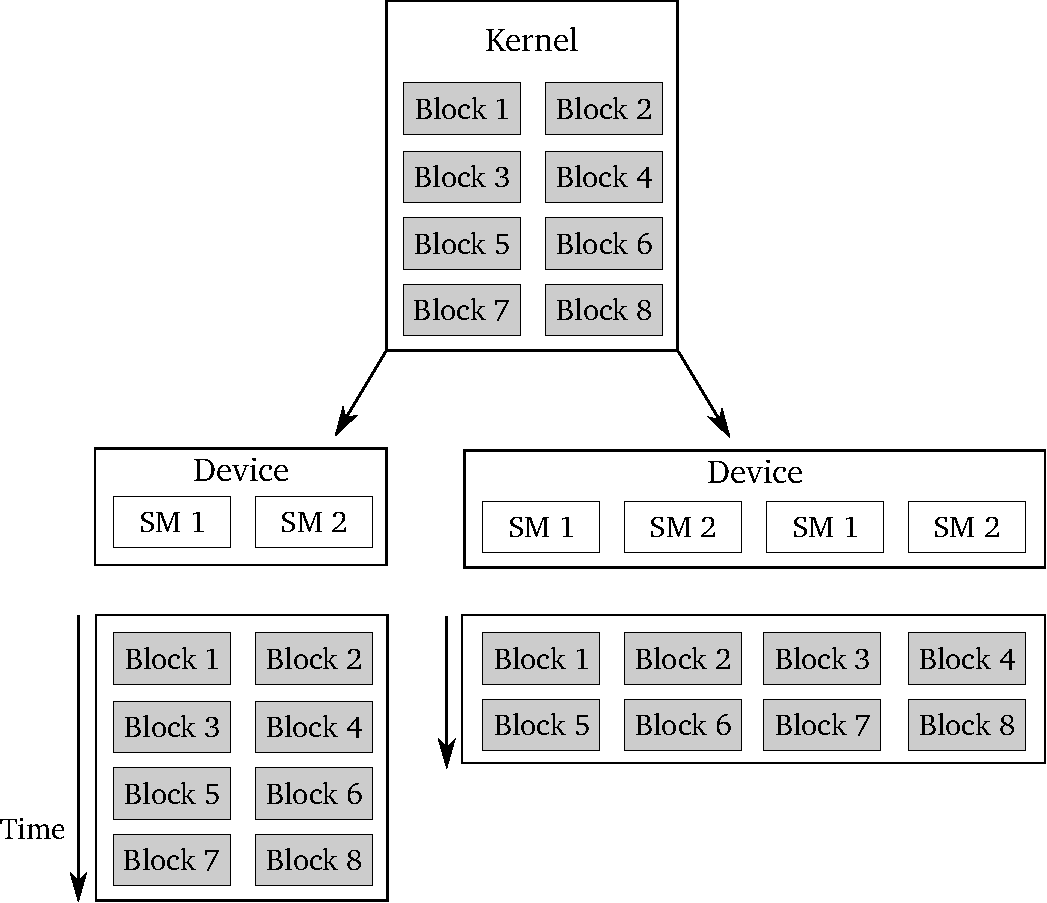
\includegraphics[scale=0.65]{Chapters/chapter1/figures/scalability.pdf}}
\caption{Scalability of GPU.}
\label{ch1:fig:scalability}
\end{figure}


A kernel is a function which  contains a block of instructions that are executed
by the  threads of a GPU.   When the problem considered  is a two  dimensional or three
dimensional  problem,  it is  possible  to group  thread  blocks  into a grid.   In
practice, the number of  thread blocks and the size of thread  blocks is given as
parameters  to  each  kernel.   Figure~\ref{ch1:fig:scalability}  illustrates  an
example of a kernel composed of 8 thread blocks. Then this kernel is executed on
a small device containing only 2 SMs.  So in  this case, blocks are executed 2
by 2 in any order.  If the kernel is executed on a larger Cuda device containing
4 SMs, blocks are executed 4 by 4 simultaneously.  The execution times should be
approximately twice faster in the latter  case. Of course, that depends on other
parameters that will be described later.

Thread blocks provide a way to cooperation  in the sense that threads of the same
block   cooperatively    load   and   store   blocks   of    memory   they   all
use. Synchronizations of threads in the same block are possible (but not between
threads of different  blocks). Threads of the same block  can also share results
in order  to compute a  single result. In chapter~\ref{chapter2},  some examples
will explicit that.


\section{Memory hierarchy}

The memory hierarchy of  GPUs\index{memory~hierarchy} is different from the CPUs
one.  In practice,  there are registers\index{memory~hierarchy!registers}, local
memory\index{memory~hierarchy!local~memory},                               shared
memory\index{memory~hierarchy!shared~memory},                               cache
memory\index{memory~hierarchy!cache~memory}              and              global
memory\index{memory~hierarchy!global~memory}.


As  previously  mentioned each  thread  can access  its  own  registers.  It  is
important to keep in mind that the  number of registers per block is limited. On
recent cards,  this number is  limited to 64Kb  per SM.  Access to  registers is
very fast, so it is a good idea to use them whenever possible.

Likewise each thread can access local  memory which, in practice, is much slower
than registers.  Local memory is automatically used by the compiler when all the
registers are  occupied. So the  best idea is  to optimize the use  of registers
even if this implies to reduce the number of threads per block.

\begin{figure}[hbtp!]
\centerline{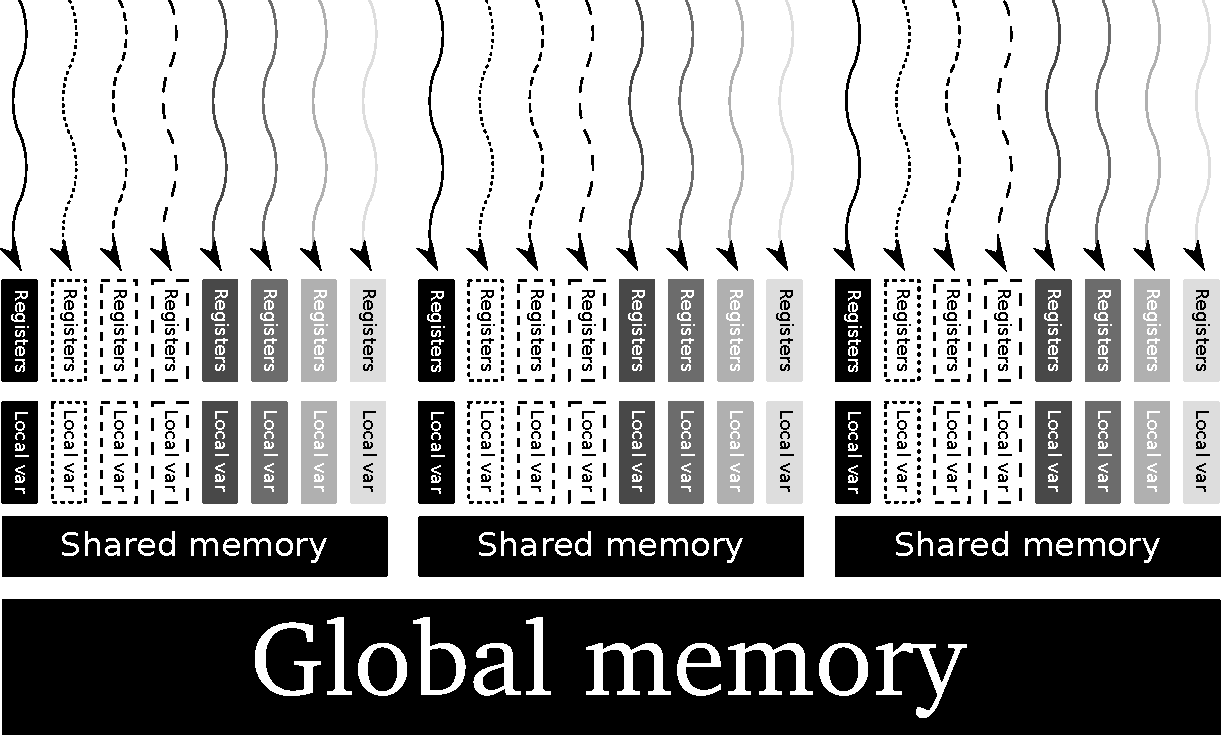
\includegraphics[scale=0.60]{Chapters/chapter1/figures/memory_hierarchy.pdf}}
\caption{Memory hierarchy of a GPU.}
\label{ch1:fig:memory_hierarchy}
\end{figure}



Shared memory allows  cooperation between threads of the  same block.  This kind
of memory is fast because it requires to be manipulated manually and its size is
limited.  It is accessible during the execution of a kernel. So the principle is
to fill the shared  memory at the start of the kernel  with global data that are
used very  frequently, then threads can  access it for  their computation.  They
can obviously change  the content of this shared  memory either with computation
or load of  other data and they can  store its content in the  global memory. So
shared memory can  be seen as a cache memory  manageable manually. This requires
obviously an effort from the programmer.

On  recent cards,  the programmer  may decide  what amount  of cache  memory and
shared memory is attributed to a kernel. The cache memory is a L1 cache which is
directly  managed by  the GPU.  Sometimes,  this cache  provides very  efficient
result and sometimes the use of shared memory is a better solution.




Figure~\ref{ch1:fig:memory_hierarchy}  illustrates  the  memory hierarchy  of  a
GPU. Threads are represented on the top  of the figure. They can access to their
own registers  and their local memory. Threads  of the same block  can access to
the shared memory of this block. The cache memory is not represented here but it
is local  to a thread. Then  each block can access  to the global  memory of the
GPU.

 \section{Conclusion}

In this chapter,  a brief presentation of the video card,  which has later been
used to perform computation, has been  given. The architecture of a GPU has been
illustrated focusing on the particularity of GPUs in term of parallelism, memory
latency and  threads. In order to design  an efficient algorithm for  GPU, it is
essential to have all these parameters in mind.


\putbib[Chapters/chapter1/biblio]


%\chapterauthor{Raphaël Couturier}{Femto-ST Institute, University of Franche-Comte}

\chapter{Introduction to Cuda}
\label{chapter2}

\section{Introduction}
\label{ch2:intro}

In this chapter  we give some simple examples of Cuda  programming.  The goal is
not to provide an exhaustive presentation of all the functionalities of Cuda but
rather to give some basic elements. Of  course, readers that do not know Cuda are
invited  to read  other  books that  are  specialized on  Cuda programming  (for
example: \cite{ch2:Sanders:2010:CEI}).


\section{First example}
\label{ch2:1ex}

This first example is  intented to show how to build a  very simple program with
Cuda.  Its goal  is to perform the sum  of two arrays and put the  result into a
third array.  A Cuda program consists in  a C code which calls Cuda kernels that
are executed on a GPU. The listing of this code is in Listing~\ref{ch2:lst:ex1}.


As GPUs have  their own memory, the first step consists  in allocating memory on
the GPU.  A call to  \texttt{cudaMalloc}\index{Cuda~functions!cudaMalloc} allows
to allocate memory on the GPU. The first parameter of this function is a pointer
on a memory on the device (i.e. the GPU). In this example, \texttt{d\_} is added
on each variable allocated  on the GPU, meaning this variable is  on the GPU. The
second parameter represents the size of the allocated variables, this size is expressed in
bits.

In this example, we  want to compare the execution time of  the additions of two
arrays in  CPU and  GPU. So  for both these  operations, a  timer is  created to
measure the  time. Cuda proposes to  manipulate timers quite  easily.  The first
step is to create the timer\index{Cuda~functions!timer}, then to start it and at
the end to stop it. For each of these operations a dedicated function is used.

In  order to  compute  the same  sum  with a  GPU, the  first  step consists  in
transferring the data from the CPU (considered as the host with Cuda) to the GPU
(considered as the  device with Cuda).  A call  to \texttt{cudaMemcpy} allows to
copy the content of an array allocated in the host to the device when the fourth
parameter                                 is                                 set
to  \texttt{cudaMemcpyHostToDevice}\index{Cuda~functions!cudaMemcpy}.  The first
parameter of the function is the  destination array, the second is the
source  array and  the third  is the  number of  elements to  copy  (expressed in
bytes).

Now the  GPU contains the  data needed to  perform the addition.   In sequential
programming, such  addition is  achieved out  with a loop  on all  the elements.
With a GPU,  it is possible to perform  the addition of all the  elements of the
two  arrays in  parallel (if  the number  of blocks  and threads  per  blocks is
sufficient).   In Listing\ref{ch2:lst:ex1}  at the  beginning, a  simple kernel,
called \texttt{addition} is defined to  compute in parallel the summation of the
two     arrays.      With     Cuda,     a     kernel     starts     with     the
keyword   \texttt{\_\_global\_\_}   \index{Cuda~keywords!\_\_shared\_\_}   which
indicates that this kernel can be called from the C code.  The first instruction
in this kernel is used to compute the variable \texttt{tid} which represents the
thread index.   This thread index\index{thread  index} is computed  according to
the           values            of           the           block           index
(called  \texttt{blockIdx} \index{Cuda~keywords!blockIdx}  in Cuda)  and  of the
thread   index   (called   \texttt{blockIdx}\index{Cuda~keywords!threadIdx}   in
Cuda). Blocks of threads and thread  indexes can be decomposed into 1 dimension,
2 dimensions or  3 dimensions.  According to the  dimension of manipulated data,
the appropriate dimension  can be useful. In our example,  only one dimension is
used.   Then using notation  \texttt{.x} we  can access  to the  first dimension
(\texttt{.y}  and \texttt{.z}  respectively allow to access  to the  second and
third dimension).   The variable \texttt{blockDim}\index{Cuda~keywords!blockDim}
gives the size of each block.



\lstinputlisting[label=ch2:lst:ex1,caption=A simple example]{Chapters/chapter2/ex1.cu}

\section{Second example: using CUBLAS}
\label{ch2:2ex}

The Basic Linear Algebra Subprograms  (BLAS) allows programmers to use efficient
routines  that are  often  required. Those  routines  are heavily  used in  many
scientific applications  and are optimized for  vector operations, matrix-vector
operations                           and                           matrix-matrix
operations~\cite{ch2:journals/ijhpca/Dongarra02}. Some  of those operations seem
to be  easy to  implement with Cuda.   Nevertheless, as  soon as a  reduction is
needed, implementing an efficient reduction routine with Cuda is far from being
simple. Roughly speaking, a reduction operation\index{reduction~operation} is an
operation  which combines  all the  elements of  an array  and extracts  a number
computed with all the  elements. For example, a sum, a maximum  or a dot product
are reduction operations.

In this second example, we consider that  we have two vectors $A$ and $B$. First
of all, we want to compute the sum  of both vectors in a vector $C$. Then we want
to compute the  scalar product between $1/C$ and $1/A$. This  is just an example
which has no direct interest except to show how to program it with Cuda.

Listing~\ref{ch2:lst:ex2} shows this example with Cuda. The first kernel for the
addition  of two  arrays  is exactly  the same  as  the one  described in  the
previous example.

The  kernel  to  compute the  opposite  of  the  elements  of  an array  is  very
simple. For  each thread index,  the inverse of  the array replaces  the initial
array.

In the main function,  the beginning is very similar to the  one in the previous
example.  First,  the user is  askef to define  the number of elements.   Then a
call  to \texttt{cublasCreate}  allows  to initialize  the  cublas library.   It
creates a handle. Then all the arrays  are allocated in the host and the device,
as in the  previous example.  Both arrays $A$ and $B$  are initialized.  The CPU
computation is performed  and the time for this CPU  computation is measured. In
order to  compute the same result  on the GPU, first  of all, data  from the CPU
need to be  copied into the memory of  the GPU. For that, it is  possible to use
cublas   function   \texttt{cublasSetVector}.    This   function   has   several
arguments. More precisely, the first  argument represents the number of elements
to transfer, the second arguments is the size of each element, the third element
represents the source  of the array to  transfer (in the GPU), the  fourth is an
offset between each element of the source  (usually this value is set to 1), the
fifth is  the destination (in the  GPU) and the  last is an offset  between each
element  of the  destination. Then  we call  the kernel  \texttt{addition} which
computes the  sum of all elements  of arrays $A$ and  $B$.  The \texttt{inverse}
kernel  is called twice,  once to  inverse elements  of array  $C$ and  once for
$A$. Finally,  we call the  function \texttt{cublasDdot} which computes  the dot
product  of two  vectors.   To use  this  routine, we  must  specify the  handle
initialized by  Cuda, the number  of elements to  consider, then each  vector is
followed by the offset between every  element.  After the GPU computation, it is
possible to check that both computation produce the same result.

\lstinputlisting[label=ch2:lst:ex2,caption=A simple example with cublas]{Chapters/chapter2/ex2.cu}

\section{Third example: matrix-matrix multiplication}
\label{ch2:3ex}



Matrix-matrix multiplication is an operation  which is quite easy to parallelize
with a GPU. If we consider that  a matrix is represented using a two dimensional
array, $A[i][j]$ represents the element of  the $i^{th}$ row and of the $j^{th}$
column. In  many cases, it is  easier to manipulate a  1D array instead  of a 2D
array.   With Cuda,  even if  it is  possible to  manipulate 2D  arrays,  in the
following we present an example based on a 1D array. For the sake of simplicity,
we  consider we  have  a square  matrix of  size  \texttt{size}.  So  with a  1D
array,  \texttt{A[i*size+j]} allows  us to  have access  to the  element  of the
$i^{th}$ row and of the $j^{th}$ column.

With  a sequential  programming, the  matrix multiplication  is  performed using
three loops. We assume that $A$, $B$  represent two square matrices and the
result   of    the   multiplication    of   $A   \times    B$   is    $C$.   The
element \texttt{C[i*size+j]} is computed as follows:
\begin{equation}
C[i*size+j]=\sum_{k=0}^{size-1} A[i*size+k]*B[k*size+j];
\end{equation}

In Listing~\ref{ch2:lst:ex3},  the CPU computation  is performed using  3 loops,
one  for $i$,  one for  $j$  and one  for $k$.   In  order to  perform the  same
computation on a  GPU, a naive solution consists in  considering that the matrix
$C$ is split into  2 dimensional blocks.  The size of each  block must be chosen
such as the number of threads per block is inferior to $1,024$.


In Listing~\ref{ch2:lst:ex3},  we consider that  a block contains 16  threads in
each   dimension,  the   variable  \texttt{width}   is  used   for   that.   The
variable \texttt{nbTh} represents the number of threads per block. So, to be able
to compute the matrix-matrix product on a GPU, each block of threads is assigned
to compute the result  of the product for the elements of  this block.  The main
part of the code is quite similar to the previous code.  Arrays are allocated in
the  CPU and  the GPU.   Matrices $A$  and $B$  are randomly  initialized.  Then
arrays are  transferred inside the  GPU memory with call  to \texttt{cudaMemcpy}.
So the first step for each thread of a block is to compute the corresponding row
and   column.    With   a    2   dimensional   decomposition,   \texttt{int   i=
blockIdx.y*blockDim.y+ threadIdx.y;} allows us to compute the corresponding line
and  \texttt{int  j=   blockIdx.x*blockDim.x+  threadIdx.x;}  the  corresponding
column. Then each  thread has to compute the  sum of the product of  the line of
$A$   by   the  column   of   $B$.    In  order   to   use   a  register,   the
kernel  \texttt{matmul}  uses a  variable  called  \texttt{sum}  to compute  the
sum. Then the result is set into  the matrix at the right place. The computation
of  CPU matrix-matrix multiplication  is performed  as described  previously.  A
timer measures  the time.   In order to  use 2 dimensional  blocks, \texttt{dim3
dimGrid(size/width,size/width);} allows us  to create \texttt{size/width} blocks
in each  dimension.  Likewise,  \texttt{dim3 dimBlock(width,width);} is  used to
create \texttt{width} thread  in each dimension. After that,  the kernel for the
matrix  multiplication is  called. At  the end  of the  listing, the  matrix $C$
computed by the GPU is transferred back  into the CPU and we check if both matrices
C computed by the CPU and the GPU are identical with a precision of $10^{-4}$.


With $1,024  \times 1,024$ matrices,  on a C2070M  Tesla card, this  code takes
$37.68$ms to perform the multiplication. With an Intel Xeon E31245 at $3.30$GHz, it
takes $2465$ms  without any parallelization (using only  one core). Consequently
the speed up  between the CPU and GPU  version is about $65$ which  is very good
regarding the difficulty of parallelizing this code.

\lstinputlisting[label=ch2:lst:ex3,caption=simple Matrix-matrix multiplication with cuda]{Chapters/chapter2/ex3.cu}

\section{Conclusion}
In this chapter, three simple Cuda examples have been  presented. They are
quite  simple. As we  cannot  present  all the  possibilities  of  the  Cuda
programming, interested  readers  are  invited  to  consult  Cuda  programming
introduction books if some issues regarding the Cuda programming are not clear.

\putbib[Chapters/chapter2/biblio]



\chapterauthor{Alan Gray and Kevin Stratford}{EPCC, The University of Edinburgh}

\chapter{Ludwig: multiple GPUs for a complex fluid lattice Boltzmann
application}

%\putbib[biblio]


\section{Introduction}
The lattice Boltzmann (LB) method (for an overview see, e.g.,
\cite{succi-book}) has become a popular approach to a variety of fluid
dynamics problems.  It provides a way to solve the incompressible,
isothermal Navier-Stokes equations and has the attractive features of
being both explicit in time and local in space. This makes the LB
method well-suited to parallel computation. Many efficient parallel
implementations of the LB method have been undertaken, typically using
a combination of distributed domain decomposition and the Message
Passing Interface (MPI). However, the potential
performance benefits offered by GPUs has motivated a new `mixed-mode'
approach to address very large problems. Here, fine-grained
parallelism is implemented on the GPU, while MPI is reserved for
larger-scale parallelism.  This mixed mode is of increasing interest
to application programmers at a time when many supercomputing services
are moving
toward clusters of GPU accelerated nodes. The design questions which
arise when developing a lattice Boltzmann code for this type of
heterogeneous system are therefore worth studying. Furthermore, similar
questions also recur in many other types of stencil-based algorithms.

The first applications of LB on GPUs were to achieve fluid-like
effects in computer animation, rather than scientific applications per
se.  These early works include simple fluids~\cite{wei2004}, miscible
two-component flow~\cite{zhu2006}, and various image processing tasks
based on the use of partial differential equations~\cite{zhao2007}.
While these early works used relatively low level graphics APIs, the
first CUDA runtime interface implementation was a two-dimensional
simple fluid problem~\cite{toelke2010}.  Following pioneering work on
clusters of GPUs coupled via MPI to study air
pollution~\cite{fan2004}, more recent work has included mixed OpenMP
and CUDA~\cite{myre2011}, Posix threads and CUDA~\cite{obrecht2011},
and MPI and CUDA for increasingly large GPU clusters
\cite{bernaschi2010,xian2011,feichtinger2011}. The heterogeneous
nature of these systems has also spurred interest in approaches
including automatic code generation \cite{walshsaar2012} and auto-tuning
\cite{williams2011} to aid application performance.

Many of these authors make use of
another attractive feature of LB: the ability to include fixed
solid-fluid boundary conditions as a straightforward addition to
the algorithm to study, for example, flow in
porous media. This points to an important
application area for LB methods: that of complex fluids.
Complex fluids include mixtures, surfactants, liquid crystals,
and particle suspensions, and typically require additional physics
beyond the bare Navier-Stokes equations to provide a full
description~\cite{aidun2010}. The representation of this extra
physics raises additional design questions for the application
programmer. Here, we consider the \textit{Ludwig} code \cite{desplat},
an LB application developed specifically for complex fluids
(\textit{Ludwig} was named for Boltzmann, 1844--1906).
We will present the steps
required to allow \textit{Ludwig} to exploit efficiently both a single
GPU, and also many GPUs in parallel.  We show that
\textit{Ludwig} scales excellently to at least the one thousand GPU level
(the largest resource available at the time of writing) with
indications that the code will scale to much larger systems as
they become available. In addition, we consider the steps required
to represent fully-resolved moving solid particles (usually referred
to as colloids in the context of complex fluids). Such particles
need to have their surface resolved on the lattice scale in order
to include relevant surface physics, and must be able to move: e.g.,
to execute Brownian motion in response to random forces from the
fluid. Standard methods are available to represent such particles
(e.g., \cite{ladd1994,nguyen2002}) which are amenable to effective
domain decomposition and message passing \cite{stratford2008}.
We describe below the additional considerations which arise
for such moving particles when developing an
implementation on a GPU.

In the following section we provide a brief overview of the lattice
Boltzmann method, and mention some of the general issues which can
influence performance in the CPU context.
In Section \ref{ch14:sec:singlegpu}, we then describe the alterations
which are required to exploit the GPU architecture effectively, and
highlight how the resulting code differs from the CPU version. In
Section \ref{ch14:sec:parallelgpu}, we extend this description to
include the steps required to allow exploitation of many GPUs in
parallel while retaining effective scaling. We also present results for
a typical benchmark for a fluid-only problem in Section
\ref{ch14:sec:parallelgpu} to demonstrate the success of the approach.
In Section \ref{ch14:sec:particles}, we describe the design choices
which are relevant to a GPU implementation of moving particles. Finally,
we include a number of general observations on software
engineering and maintenance which arise from our experience.
A summary is provided in Section~\ref{ch14:sec:summary}.


\section{Background}\label{ch14:sec:background}

%\begin{figure}[!t]
%\centering
%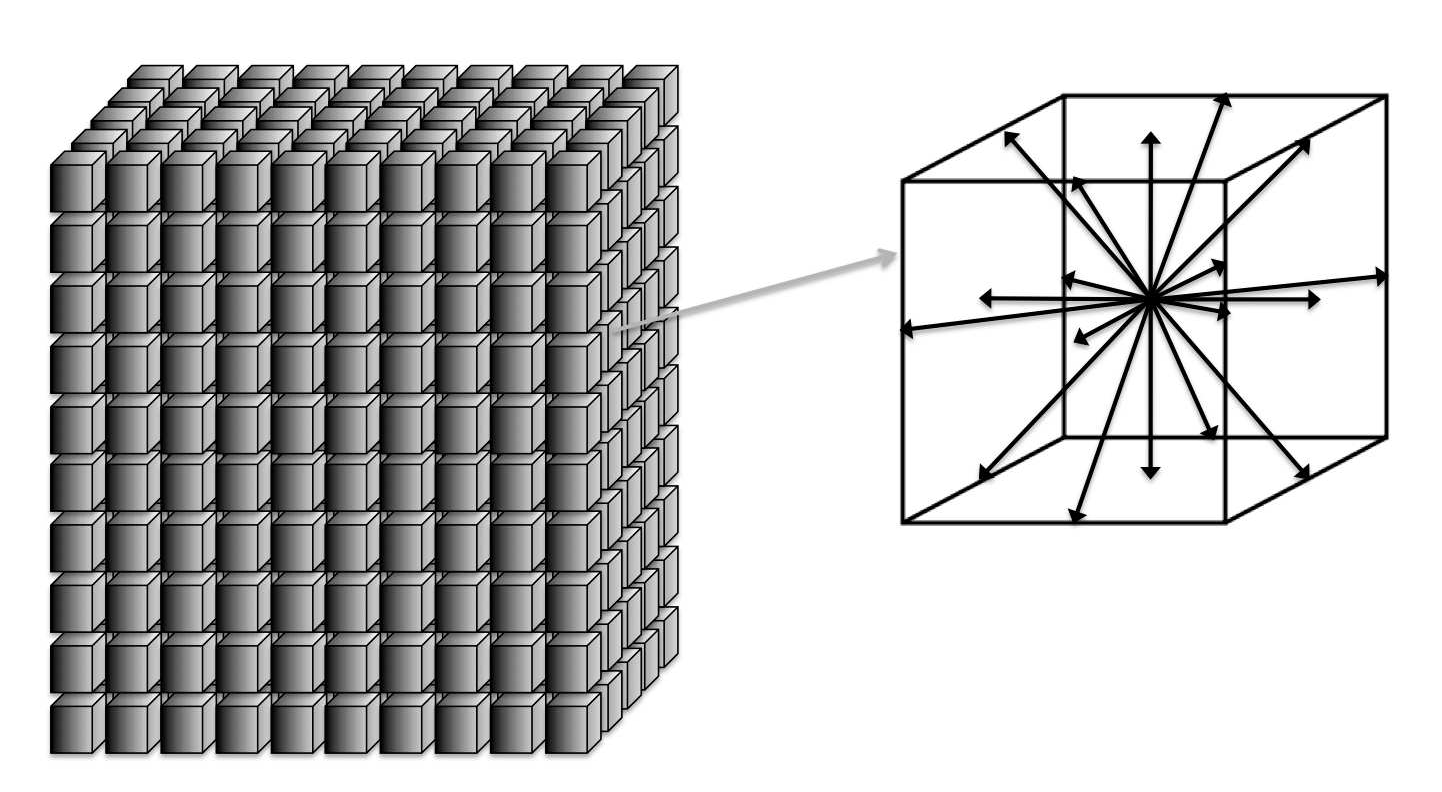
\includegraphics[width=12cm]{Chapters/chapter14/figures/basiclattice}
%\caption{The lattice Boltzmann approach discritises space into a 3D lattice (left). The fluid is represented at each lattice site (right), by the {\it distribution} vector: each component corresponding to a specific velocity direction. Here we are interested in the {\it D3Q19} model, in which there are 3 spatial directions and 19 velocity components (including a zero component).}
%\label{ch14:fig:basiclattice}
%\end{figure}


For a general complex fluid problem the starting point is the
fluid velocity field $\mathbf{u}(\mathbf{r})$, whose evolution
obeys the Navier-Stokes equations describing the conservation of mass
(or density $\rho$), and momentum:
\begin{equation}
\rho  [ \partial_t \mathbf{u} + (\mathbf{u}.\mathbf{\nabla})\mathbf{u} ]
= -\nabla p + \eta \nabla^2 \mathbf{u} + \mathbf{f}(\mathbf{r}),
\end{equation}
where $p$ is the isotropic pressure and $\eta$ is the viscosity.
A local force $\mathbf{f}(\mathbf{r})$ provides a means for coupling
to other complex fluid constituents, e.g., it might represent the force
exerted on the fluid by a curved interface between different phases or
components.

The LB approach makes use of a regular three-dimensional
lattice (see Figure \ref{ch14:fig:decomphalo}) with discrete spacing
$\Delta r$. It also makes use of a
discrete velocity space $\mathbf{c}_i$, where the $\mathbf{c}_i$
are chosen to capture the correct symmetries of the Navier-Stokes
equations. A typical choice, used here, is the so-called D3Q19
basis in three dimensions where there is one velocity such that
$\mathbf{c} \Delta t$ is zero, along with six extending to the nearest
neighbour
lattice sites, and twelve extending to the next-nearest neighbour sites
($\Delta t$ being the discrete time step). The fundamental object
in LB is then the distribution function $f_i (\mathbf{r};t)$ whose
moments are related to the local hydrodynamic quantities: the fluid
density, momentum, and stress. The time evolution of the distribution
function is described by a discrete Boltzmann equation
\begin{equation}
f_i(\mathbf{r} + \mathbf{c}_i \Delta t; t) - f_i(\mathbf{r}; t) 
= - {\cal L}_{ij} f_j(\mathbf{r};t).
\end{equation}
It is convenient to think of this in two stages. First, the right hand
side represents the action of a collision operator ${\cal L}_{ij}$,
which is local to each lattice site and relaxes the distribution toward
a local equilibrium at a rate ultimately related to the fluid viscosity.
Second, the left hand side represents a propagation step (sometimes referred
to as streaming step), in which each element $i$ of the distribution is
displaced $\mathbf{c}_i \Delta t$, i.e., one lattice spacing in the
appropriate direction per discrete time step. 

More specifically, we store a vector of 19 double precision floating
point values at each lattice site for the distribution function
$f_i(\mathbf{r};t)$.
The collision operation ${\cal L}_{ij}$, which is local at each lattice
site, may be thought of as follows. A matrix-vector multiplication
${\cal M}_{ij}f_j$ is used to transform the distributions into the
hydrodynamic quantities, where ${\cal M}_{ij}$ is a constant 19x19
matrix related to the choice of
$\mathbf{c}_i$. The non-conserved hydrodynamic quantities are then
relaxed toward their (known) equilibrium values, and are transformed
back to new post-collision distributions via the inverse transformation
${\cal M}^{-1}_{ij}$. This gives rise to the need for a minimum of 2x19$^2$
floating point multiplications per lattice site. (Additional operations are
required to implement, for example, the force $\mathbf{f}(\mathbf{r})$.)
In contrast, the
propagation stage consists solely of moving the distribution values
between lattice sites, and involves no floating point operations.

In the CPU version, the \textit{Ludwig} implementation stores one time
level of distribution values $f_i(\mathbf{r}; t)$. This distribution
is stored as a flat array of C data type \texttt{double}, and laid out
so that all elements of the velocity are contiguous at a given site
(often referred to as ``array-of-structures'' order). This is
appropriate for sums over the distribution required locally at the
collision stage as illustrated schematically in
Listing~\ref{ch14:listing1}: the fact that consecutive loads are from
consecutive memory addresses allows the prefetcher to engage fully.
(The temporary scalar \texttt{a\_tmp} allows caching of the
intermediate accumulated value in the innermost loop.)  A variety of
standard sequential optimisations are relevant for the collision stage
(loop unrolling, inclusion of SIMD operations, and so on
\cite{wellein2006}).  For example, the collision stage in
\textit{Ludwig} includes explicit SIMD code, which is useful if the
compiler on a given platform cannot identify it.  The propagation
stage is separate, and is organised as a ``pull'' (again, various
optimisation have been considered, e.g.,
\cite{pohl2003,mattila2007,wittmann2012}).  No further optimisation is
done here beyond ensuring that the ordering of the discrete velocities
allows memory access to be as efficient as possible. While these
optimisations are important, it should be remembered that for some
complex fluid problems, the hydrodynamics embodied in the LB
calculation is a relatively small part of the total computational cost
(at the 10\%-level in some cases).  This means optimisation effort may
be better concentrated elsewhere.

\begin{lstlisting}[float, label=ch14:listing1,
caption = Collision schematic for CPU.]
/* loop over lattice sites */
for (is = 0; is < nsites; is++) {
  ...
  /* load distribution from ``array-of-structures'' */
  for (i = 0; i < 19; i++)    
    f[i] = f_aos[19*is + i]
  ...
  /* perform matrix-vector multiplication */  
  for (i = 0; i < 19; i++) {    
    a_tmp = 0.0;    
    for (j = 0; j < 19; j++) {      
      a_tmp += f[j]*M[i][j];   
    }
    a[i] = a_tmp;
  }
  ...
}
\end{lstlisting}


\begin{figure}[!t]
\centering
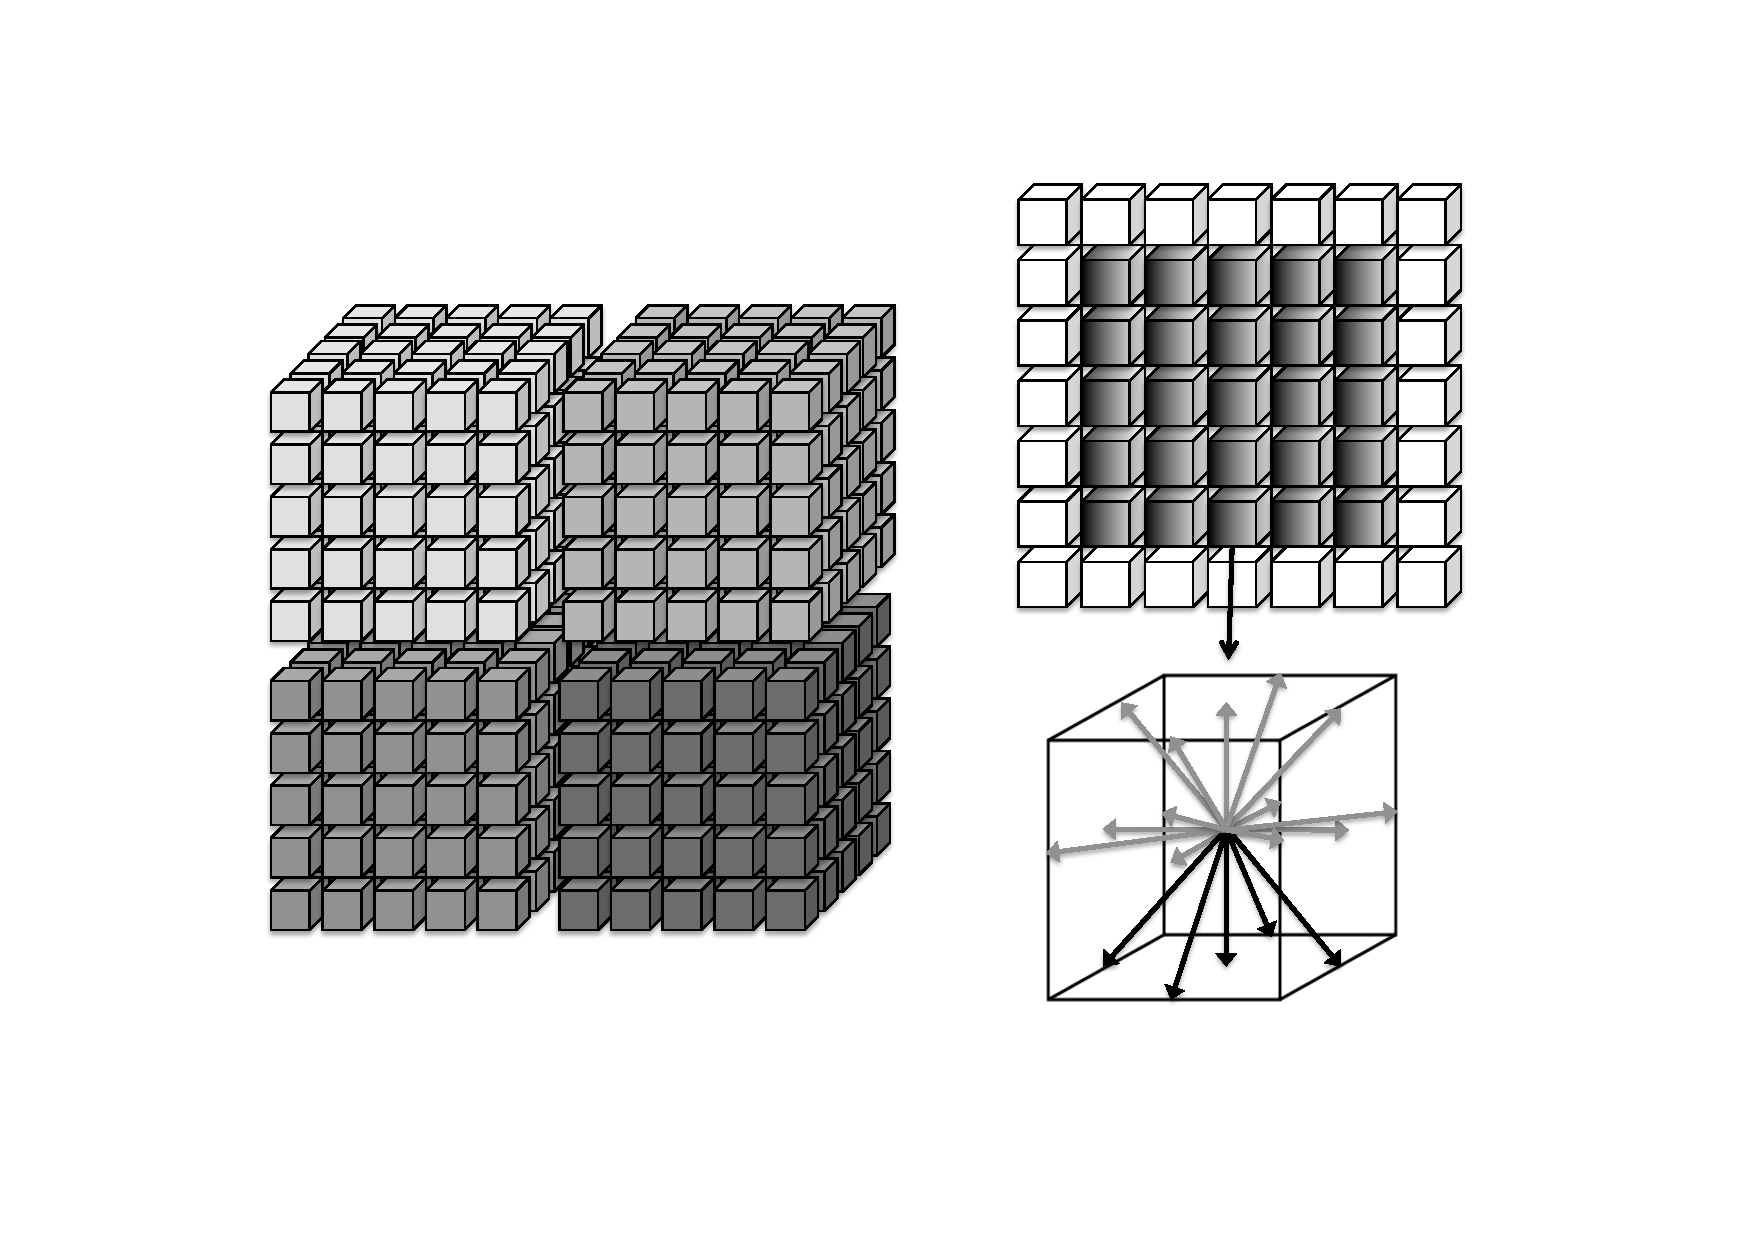
\includegraphics[width=12cm]{Chapters/chapter14/figures/decomphalo}
\caption{Left: the lattice is decomposed between MPI tasks. For
  clarity we show a 2D decomposition of a 3D lattice, but in practice
  we decompose in all 3 dimensions. Halo cells are added to each
  sub-domain (as shown on the upper right for a single slice) which store
  data retrieved from remote neighbours in the halo exchange. Lower
  right: the D3Q19 velocity set resident on a lattice site;
  highlighted are the 5 ``outgoing'' elements to be transferred in a
  specific direction.}
\label{ch14:fig:decomphalo}
\end{figure}


The regular 3D decomposition is illustrated in Fig.~\ref{ch14:fig:decomphalo}.
Each local sub-domain is surrounded by a halo, or ghost, region of width one
lattice site. While the collision is local, elements of the distribution
must be exchanged at the edges of the domains to facilitate the propagation.
To achieve the full 3D halo exchange, the standard approach of shifting the
relevant data in each co-ordinate direction in turn is adopted. This
requires appropriate synchronisation, i.e., a receive in the the first
co-ordinate direction must be complete before a send in the second direction
involving relevant data can take place, and so on. We note that only
``outgoing'' elements of the distribution need to be sent at each edge.
For the D3Q19 model, this reduces the volume of data traffic from 19 to
5 of the $f_i(\mathbf{r};t)$ per lattice site at each edge. In the CPU
version, the necessary transfers are implemented in place using
a vector of appropriately strided MPI datatypes for each direction.


\section{Single GPU Implementation}\label{ch14:sec:singlegpu}


In this section we describe the steps taken to enable \textit{Ludwig}
for the GPU. There are a number of crucial issues: first, the
minimisation of data traffic between host and device; second, the
optimal mapping of available parallelism onto the architecture and
third, the issue of memory coalescing. We discuss each of these in
turn.

While the most important section of the LB in terms of
floating-point performance is the collision stage, this cannot be the
only consideration for a GPU implementation. It is essential to
offload all computational activity which involves the main data
structures (such as the distribution) to the GPU. This includes
kernels with relatively low computational demand, such as the
propagation stage. All relevant data then remain resident on the GPU,
to avoid expensive host-device data transfer at each iteration of
the algorithm. Such transfers would negate any benefit of GPU
acceleration.  We note that for a complex fluid code, this requirement
can extend to a considerable number of kernels, although we limit the
discussion to collision and propagation for brevity.

To achieve optimal performance, it is vital to exploit fully the
parallelism inherent in the GPU architecture, particularly for
those matrix-vector operations within the collision kernel.
The GPU architecture features a hierarchy of parallelism. At the
lowest level, groups of 32 threads (warps) operate in
lock-step on different data elements: this is SIMD style vector-level
parallelism. Multiple warps are combined into a thread block (in which
communication and synchronisation are possible), and multiple blocks can
run concurrently across the streaming multiprocessors in the GPU
(with no communication or
synchronisation possible across blocks).  To decompose on the GPU, we
must choose which part of the collision to assign to which level of
parallelism.

While there exists parallelism within the matrix-vector operation, the
length of each vector (here, 19) is smaller than the warp size and typical
thread block sizes. So we simply decompose the loop over lattice sites
to all levels of parallelism, i.e., we use a separate CUDA thread for
every lattice site, and each thread performs the full matrix-vector
operation. We find that a block size of 256 performs well on current
devices: we therefore decompose
the lattice into groups of 256 sites, and assign each group to a block
of CUDA threads. As the matrix ${\cal M}_{ij}$ is constant, it is
assigned to the fast {\it constant} on-chip device memory.

For the propagation stage, the GPU implementation adds a second time
level of distribution values. The data-dependencies inherent in the
propagation mean that the in-place propagation of the CPU version
cannot be parallelised effectively without the additional time level.
As both time levels may remain resident on the GPU, this is not a
significant overhead.

An architectural
constraint of GPUs means that optimal global memory bandwidth
is only achieved when data are structured such that threads within a
{\it half-warp} (a group of 16 threads) load data from the same memory
segment in a single transaction: this is memory coalescing. It can be
seen that the array-of-structures ordering used for the distribution
in the CPU code would not be suitable for coalescing; in fact, it would
result in serialised memory accesses and relative poor performance.
To meet the coalescing criteria and allow consecutive threads to read
consecutive memory addresses on the GPU, we transpose the layout of the
distribution so that, for each velocity component, consecutive sites
are contiguous in memory (``structure-of-arrays'' order). A schematic of
the GPU collision code is given in Listing~\ref{ch14:listing2}.

\begin{lstlisting}[float, label=ch14:listing2,
caption = Collision schematic for GPU.]
/* compute current site index 'is' from CUDA thread and block */
/* indices and load distribution from "structure-of-arrays" */

for (i = 0; i < 19; i++)    
  f[i] = f_soa[nsites*i + is]

/* perform matrix-vector multiplication as before */
...
\end{lstlisting}


\textit{Ludwig} was modified to allow a choice of distribution data layout
at compilation time depending on the target architecture: CPU or GPU. We
defer some further comments on software engineering aspects of the code to
the summary.


\section{Multiple GPU Implementation}\label{ch14:sec:parallelgpu}

To execute on multiple GPUs, we use the same domain decomposition
and message passing framework as the CPU version. Within each
sub-domain (allocated to one MPI task) the GPU implementation
proceeds as described in the previous section. The only additional
complication is that halo transfers between GPUs must be staged
through the host (in future, direct GPU to GPU data transfers via
MPI may be possible, obviating the need for these steps). This
means host MPI sends must be preceded by appropriate device to host
transfers and host MPI receives must be followed by corresponding host
to device transfers.

%To execute on multiple GPUs in parallel we decompose the problem using
%the existing high-level parallelisaton framework: each MPI task acts
%as a host to a separate GPU, with each GPU kernel operating on the
%subset of the lattice volume corresponding to the partition assigned
%to that task.  As described in Section \ref{ch14:sec:background}, halo
%data exchanges are required at each timestep.  Significant
%developments are made for the GPU adaptation of this communication
%phase to achieve good inter-GPU communication performance and allow
%scaling to many GPUs.

%The CPU code uses strided MPI datatypes to define the six
%planes of lattice data to be sent or received, and performs the
%communications {\it in-place}, i.e.  there is no explicit buffering of
%data in the application.  For the GPU adaptation, the halo planes must
%be exchanged between GPUs, on which MPI functionality is not
%available, so transfers must be staged through the host CPUs. Buffer
%packing/unpacking of the halo planes is explicitly performed using
%CUDA kernels, and CUDA memory copy calls are used to transfer data
%from a device to its host (using pinned host memory) through the PCI-e
%bus (and vice versa). MPI calls are used to transfer the buffers
%between hosts. The CPU version of Ludwig has a mechanism, using MPI built-in
%data types, to reduce the amount of data communicated by around a
%factor of four by only sending those elements of the distribution
%propagating outward from a local domain. For the GPU adaptation, this
%filtering of data is explicitly performed (again since MPI
%functionality is not available on the GPU) in the buffer
%packing/unpacking kernels.  Special care had to be taken for those
%lattice sites on the corners of the halo planes, which had to be sent
%in more than one direction (since the propagation includes accesses to
%diagonal neighbours).

In practice, this data movement requires additional GPU kernels to
pack and unpack the relevant data before and after corresponding MPI
calls. However, the standard shift algorithm, in which each co-ordinate
direction is treated in turn, does provide some scope for the
overlapping of different operations.
For example, after the data for the first co-ordinate direction have been
retrieved by the host, these can be exchanged using MPI between
hosts at the same time as kernels for packing and retrieving of
data for the second co-ordinate direction are
executed. This
overlapping must respect the synchronisation required to ensure
that data values at the corners of the sub-domain are transferred
correctly.
We use a separate CUDA stream for each co-ordinate direction:
this allows some of the host-device communication time to be
effectively ``hidden'' behind the host-host MPI communication,
resulting in an overall speedup.
The improvement is more pronounced for the smaller local lattice size,
perhaps because of less CPU memory bandwidth contention. The
overlapping is then a particularly valuable aid to strong scaling,
where the local system size decreases as the number of GPUs increases.


%\section{Performance}\label{ch14:sec:performance}

To demonstrate the effectiveness of our approach, we compare the
performance of both CPU and GPU versions of \textit{Ludwig}. To
test the complex fluid nature of the code, the problem is
actually an immiscible fluid mixture which uses a second distribution
function to introduce a composition variable. The interested reader
is referred to \cite{ch14:stratford-jsp2005} for further details. The
largest total problem size used is $2548\times 1764\times 1568$.
The CPU system features a Cray XE6 architecture with 2 16-core AMD Opteron
CPUs per node, and with nodes interconnected using Cray Gemini technology.
For GPU results, a Cray XK6 system is used: this is very similar to the
XE6, but has one CPU per node replaced with an NVIDIA X2090 GPU. Each
node in the GPU system therefore features a single Opteron CPU acting
as a host to a single GPU. The inter-node interconnect architecture is
the same as for the Cray XE6. The GPU performance tests use a prototype
Cray XK6 system with 936 nodes (the largest available at the time of writing).
To provide a fair comparison, we compare scaling on a \textit{per node}
basis. That is, we compare 1 fully occupied 32-core CPU node
(running 32 MPI tasks) with 1 GPU node (host running 1 MPI task,
and 1 device). We believe this is representative of the true ``cost'' of
a simulation in terms of accounting budgets, or electricity.


%\begin{figure}[!t]
%\centering
%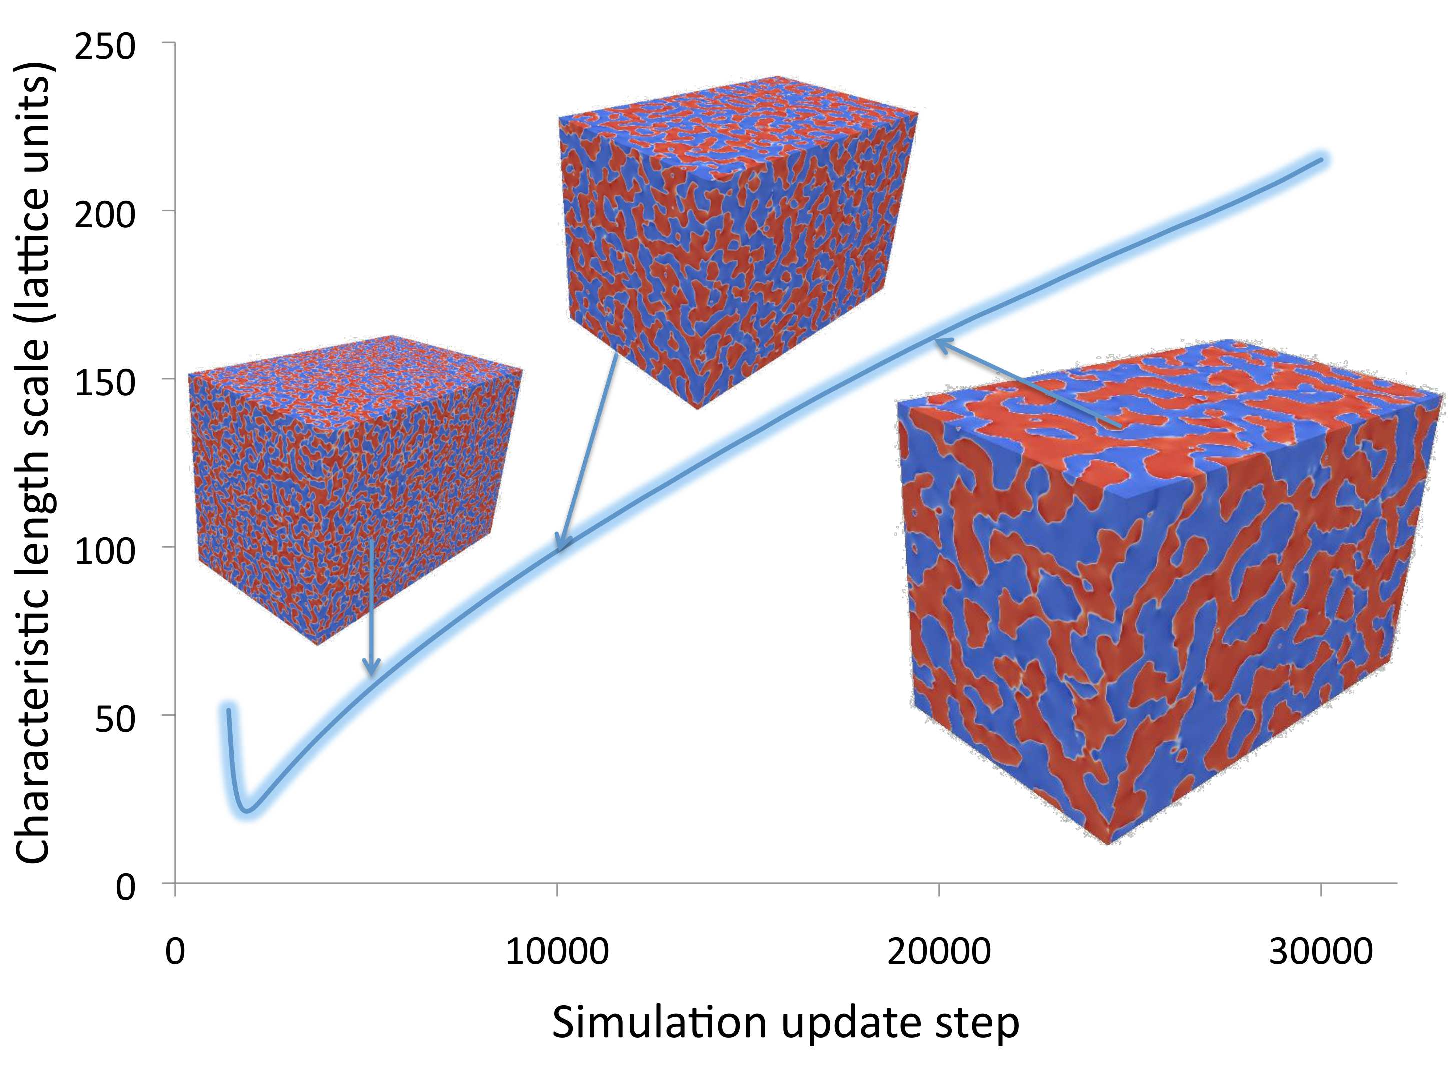
\includegraphics[width=10cm]{Chapters/chapter14/figures/length_scale}
%\caption{The dependence of the characteristic length scale of a binary
%  fluid mixture on the simulation timestep number. Superimposed are
%  three snapshots showing increased mixture separation with time:
%  these are obtained through the order parameter and each show one
%  eighth of the total simulation size, which is $1548\times 1764\times 1568$. }\label{ch14:fig:length_scale}
%\end{figure}  

\begin{figure}[!t]
\centering
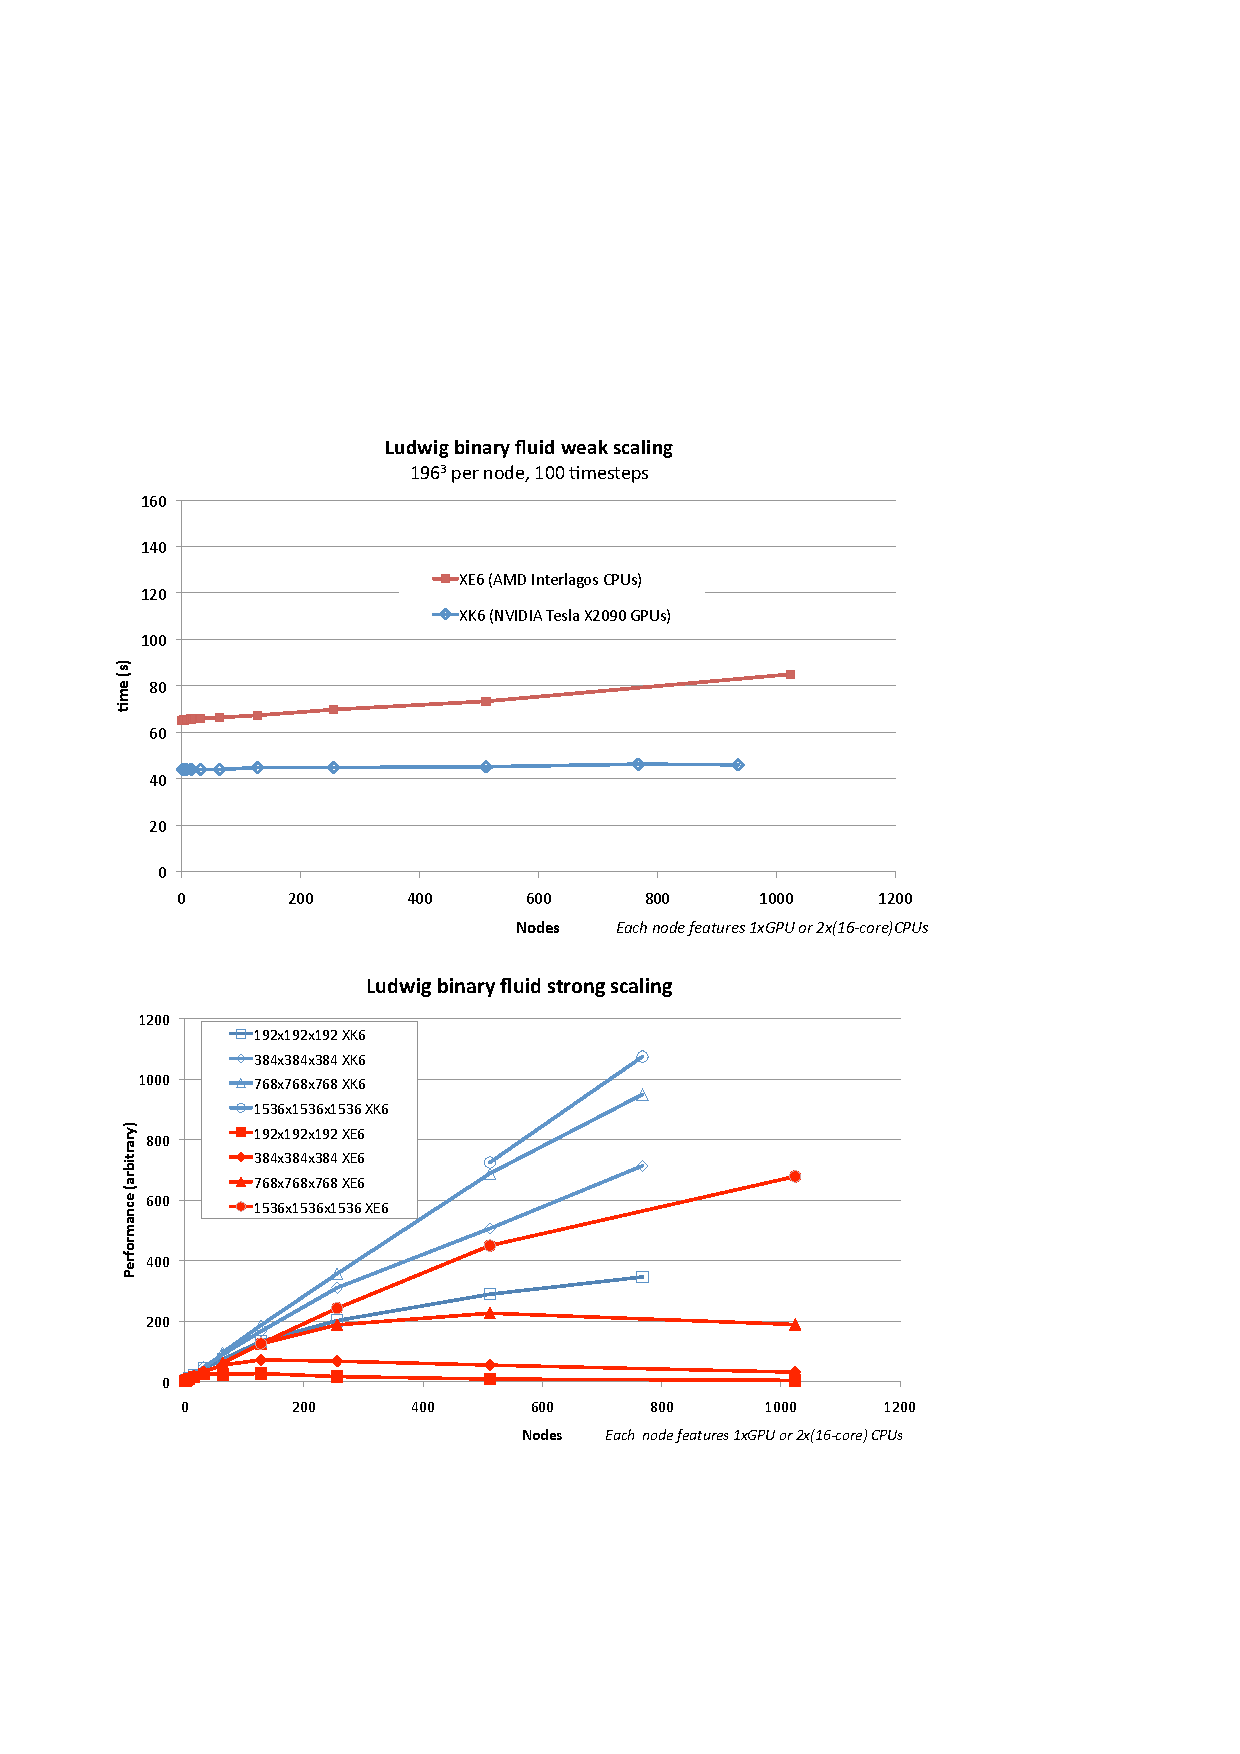
\includegraphics[width=10cm]{Chapters/chapter14/figures/two_graphs_ud}
\caption{The weak (top) and strong (bottom) scaling of \textit{Ludwig}.  Closed
  shapes denote results using the CPU version run on the Cray
  XE6 (using two 16-core AMD Interlagos CPUs per node), while open
  shapes denote results using the GPU version on the Cray XK6 (using a
  single NVIDIA X2090 GPU per node). Top: the benchmark time is shown
  where the problem size per node is constant. Bottom: performance is
  shown where, for each of the four problem sizes presented, the
  results are scaled by the lattice volume, and all results are
  normalized by the same arbitrary constant.  }
\label{ch14:fig:scaling}
\end{figure}


%The top of Figure \ref{ch14:fig:scaling} shows the benchmark time,
%where the problem size is increased with the number of nodes. This
%shows weak scaling: the time taken by a perfectly scaling code would
%remain constant. The figure plots the time against the number of {\it
%  nodes}: for the GPU version we utilize the one GPU per Cray XK6 node
%whilst for the CPU version we fully utilize two 16-core CPUs
%per Cray XE6 node, i.e. one GPU is compared with 32 CPU cores.  We use
%a single MPI task per Cray XK6 node to host the GPU, and 32 MPI tasks
%to fully utilize the CPUs in the Cray XE6 node.  Note that our CPU
%version is highly optimised: in particular it has been tuned for
%optimal utilisation of the SIMD vector units in each CPU core.

Figure \ref{ch14:fig:scaling} shows the results of both weak and
strong scaling tests (top and bottom panels, respectively). For
weak scaling, where the local sub-domain size is kept fixed
(here a relatively large 196$^3$ lattice), the time taken by
an ideal code would remain constant. It can be seen that while
scaling of the CPU version shows a pronounced upward slope, the
GPU version scales almost perfectly. The advantage of the GPU
version over the CPU version is the fact that the GPU version
has a factor of 32 fewer MPI tasks per node, so communications
require a significantly smaller number of larger data transfers.
The performance
advantage of the GPU version ranges from a factor of around 1.5 to
around 1.8. Careful study by other authors \cite{williams2011} have
found the absolute performance (in terms of floating point
operations per second, or floating point operations per Watt) to
be remarkably similar between architectures.

Perhaps of more interest is the strong scaling picture (lower
panel in Figure \ref{ch14:fig:scaling}) where the performance
as a function of the number of nodes is measured for fixed problem
size. We consider four different fixed problem sizes on both CPU
(up to 512 nodes shown) and GPU (up to 768 nodes). To allow comparison,
the results are scaled by total system size in each case. For strong
scaling, the disparity in the number of MPI tasks is clearly revealed
in the failure of the CPU version to provide any significant benefit
beyond a modest number of nodes as communication overheads dominate.
In contrast, the GPU version shows
reasonably robust scaling even for the smaller system sizes and good
scaling for the larger systems.

\section{Moving Solid Particles}\label{ch14:sec:particles}

\begin{figure}[t]
\centering
%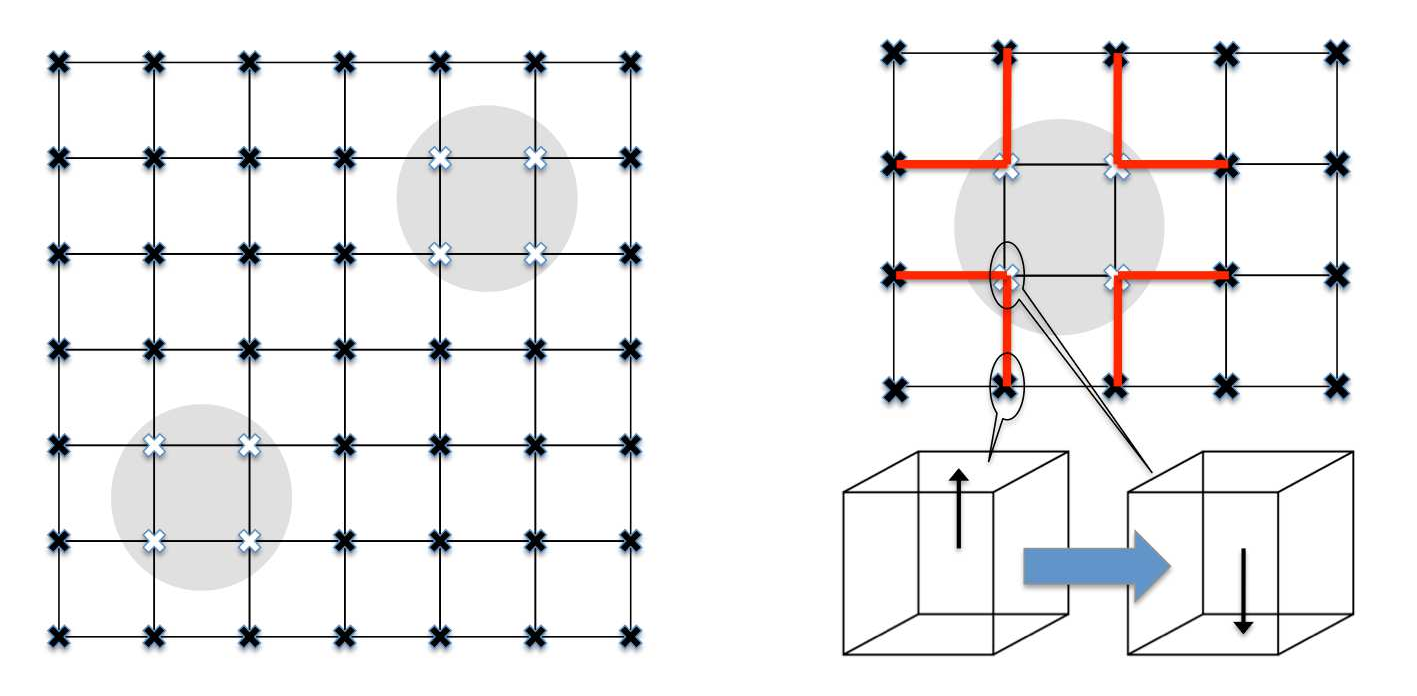
\includegraphics[width=10cm]{Chapters/chapter14/figures/bbl}
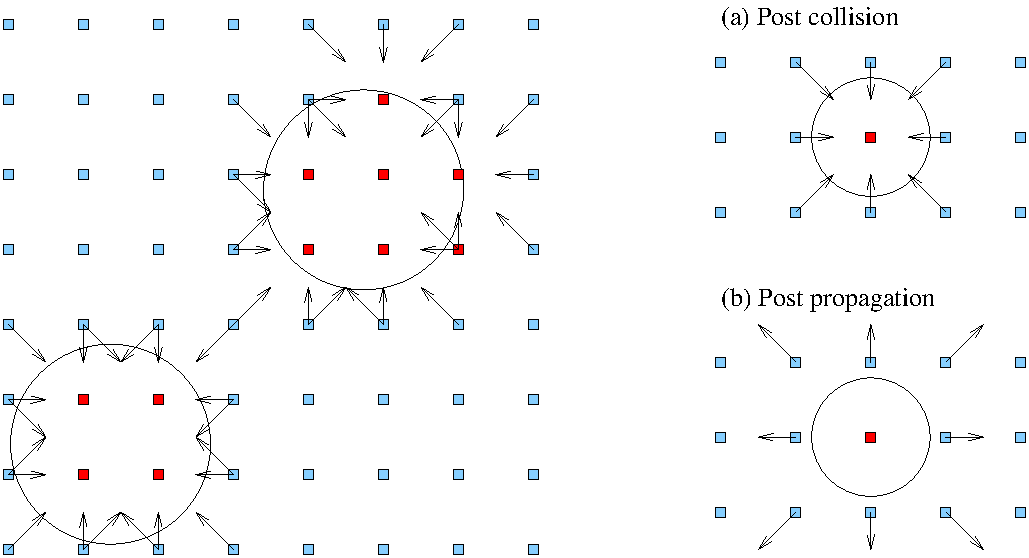
\includegraphics[width=10cm]{Chapters/chapter14/figures/colloid_new}
\caption{
A two-dimensional schematic picture of spherical particles on the lattice.
Left: a particle is allowed
to move continuously across the lattice, and the position of the
surface defines fluid lattice sites (light blue) and solid lattice
sites (dark red). The discrete surface is defined by links
where propagation would intersect the surface (arrows). Note the
discrete shape of the two particles is different. Right: post-collision
distributions are reversed at the surface by the process of bounce-back
on links, which replaces the propagation.
%A 2D illustration of colloidal particles (grey circles)
%  interacting with the lattice, where each lattice point is
%  represented by a cross. Left: each particle spans multiple sites.
%  Right: the particle-facing distribution components are moved inside
%  the particle with the direction reversed, such that the ``bounce
%  back'' will be completed when the fluid propagates.
}
\label{ch14:fig:bbl}
\end{figure}


%\begin{figure}[t]
%\centering
%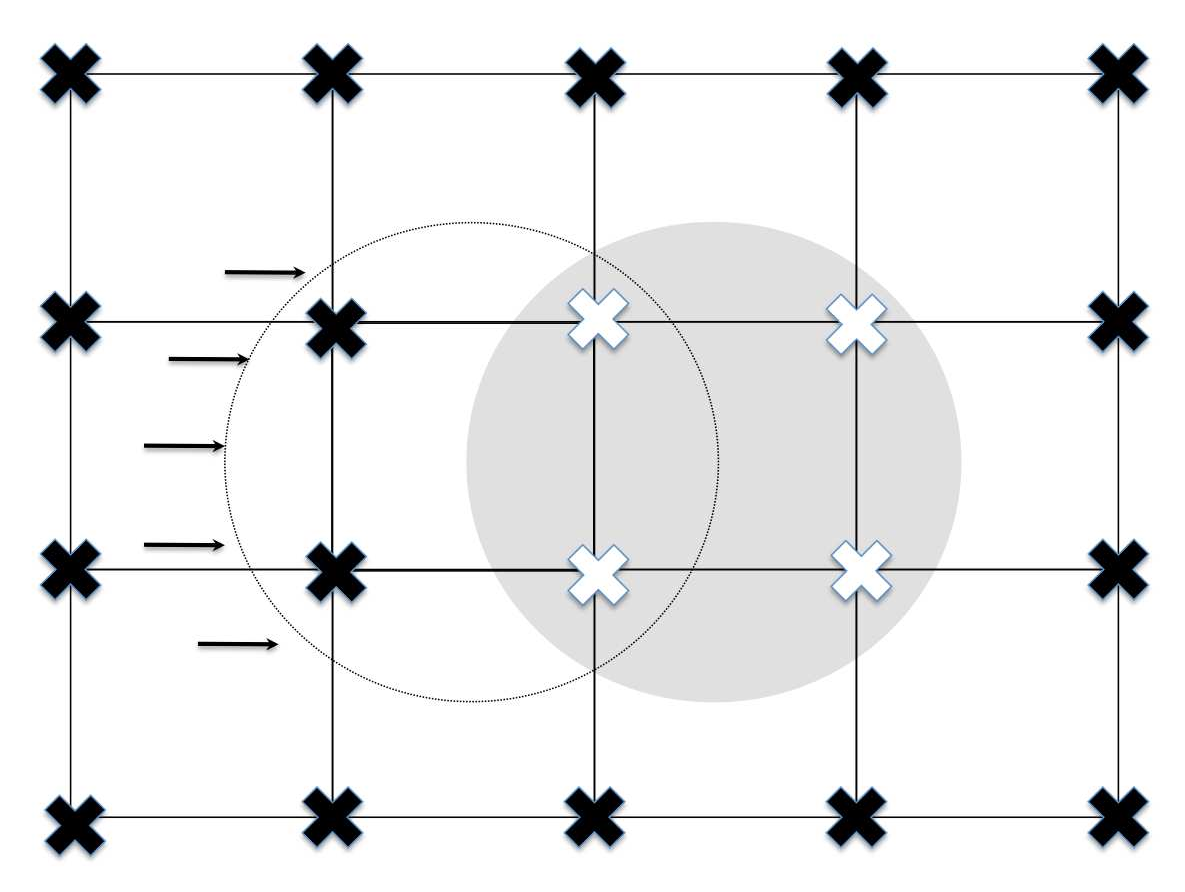
\includegraphics[width=6cm]{Chapters/chapter14/figures/particlemove}
%\caption{A 2D illustration of a colloidal particle moving across the
%    lattice. The old and new positions are represented by the open and
%    filled circles respectively.}
%\label{ch14:fig:particlemove}
%\end{figure}

% BEING NEW SOLID TEXT

The introduction of moving solid particles poses an additional hurdle
to efficient GPU implementation of an LB code such as \textit{Ludwig}.
In this section, we give a brief overview of the essential features
of the CPU implementation, and how the considerations raised in the
previous sections --- maximising parallelism and minimising both
host to device and GPU to GPU data movement --- shape the design decisions
for a GPU implementation. We restrict our discussion to a simple fluid
in this section; additional solid-fluid boundary conditions (e.g.,
wetting at a fluid-fluid-solid contact line) usually arise elsewhere
in the calculation and broadly independent of the hydrodynamic boundary
conditions which are described in what follows.

Moving solid particles (here, spheres) are defined by a centre position
which is allowed to move continuously across the space of the lattice,
and a fixed radius which is typically a few lattice spacings $\Delta r$.
The surface of the particle is defined by a series of \textit{links}
where a discrete velocity propagation $\mathbf{c}_i \Delta t$ would
intercept or cut the spherical shell (see Fig.~\ref{ch14:fig:bbl}).
Hydrodynamic boundary conditions are then implemented via the standard
approach of bounce-back on links \cite{ladd1994, nguyen2002}, where the
relevant post-collision distribution values are reversed at the
propagation stage with an appropriate correction to allow for the
solid body motion. The exchange of momentum at each link must then be
accumulated around the entire particle surface to provide the net
hydrodynamic force
and torque on the sphere. The particle motion can then be updated in a
molecular dynamics-like step.

For the CPU implementation, a number of additional MPI communications
are required: (1) to exchange the centre position, radius, etc of each
particle as it moves and (2), to allow the accumulation of the force
and torque for each particle (the links of which may be distributed
between up to 8 MPI tasks in three dimensions). Appropriate marshaling
of these data can provide an effective parallelisation for relatively
dense particle suspensions of up to  40\% solid volume fraction
\cite{stratford2008}. As a final consideration, fluid distributions
must be removed and replaced consistently as a given particle moves
across the lattice and changes its discrete shape.

With these features in mind, we can identify a number of competing
concerns which are relevant to a GPU implementation:
\begin{enumerate}
\item
Minimisation of host-device data transfer would argue for moving the
entire particle code to the GPU. However, the code in question involves
largely conditional logic (e.g., identifying cut surface links) and
irregular memory accesses (e.g., access to distribution elements around
a spherical particle). These operations seem poorly suited to effective
parallelisation on the GPU. As an additional complication, the sums
required over the particle surface would involve potentially tricky
and inefficient reductions in GPU memory.
\item
The alternative is to retain the relevant code on the CPU. While the
transfer of the entire distribution $f_i(\mathbf{r};t)$ between host
and device at each time step is unconscionable owing to PCIe bus bandwidth
considerations, the transfer of only relevant distribution information
to allow bounce-back on links is possible. At modest solid volumes
only a very small fraction of the distribution data is
involved in bounce-back (e.g., a 2\% solid volume fraction of particles
radius 2.3$\Delta r$ would involve approximately 1\% of the distribution
data). This option also has the advantage that no further host-device
data transfers are necessary to allow the MPI exchanges required for
particle information.
\end{enumerate}


We have implemented the second option as follows. For each sub-domain,
a list of boundary-cutting links is assembled on the CPU which includes
the identity of the relevant element of the distribution. This list,
together with the particle information required to compute the correct
bounce-back term, are transferred to the GPU. The updates to the relevant
elements of the distribution can then take place on the GPU. The
corresponding information to compute the update of the particle dynamics
is returned
to the CPU, where the reduction over the surface links is computed.
The change of particle shape may be dealt with in a similar manner:
the relatively small number of updates required at any one time step
(or however frequently the particle position is updated) can be
marshaled to the GPU as necessary. This preliminary implementation
is found to be effective on problems involving up to 4\%
solid volume fraction.

We note that the CPU version actually avoids the collision calculation
at solid lattice points by consulting a look-up table of solid/fluid
status. On the GPU, it is perhaps preferable to perform the collision
stage everywhere instead of moving the look-up table to the GPU and
introducing the associated logic.
Ultimately, the GPU might favour other boundary methods which treat solid and
fluid on a somewhat more equal basis, for example, the immersed boundary
method \cite{ch14:immersed,ch14:immersed-lb} or smoothed profile method
\cite{ch14:spm}.
However, the approach adopted here  allows us to exploit
the GPU for the intensive fluid simulation whilst maintaining the complex
code required for particles on the CPU. Overheads of CPU-GPU transfer are
minimised by transferring only those data relevant to the hydrodynamic
interaction implemented via bounce-back on links.

% END NEW SOLID TEXT

%It is of interest, in many situations, to include colloidal particles
%in the simulation **more from Kevin***. These are by represented by
%moving spheres that interact with the fluid through transfer of
%momenta: fluid coming into contact with a particle will bounce off it,
%giving the particle a kick in the process. As illustrated on the left
%of Figure \ref{ch14:fig:bbl} (which shows 2 dimensions only for
%clarity - in practice, the particles will be represented by spheres on
%a 3D lattice, and will be much larger relative to the lattice
%spacing), typically each particle spans multiple lattice sites, and
%therefore ``intercepts'' multiple inter-site links. Ludwig stores
%particle information using nested linked lists: a list of particles,
%each with a list of all the links intercepted by that particle (plus
%other quantities). The fluid-particle interaction proceeds using the
%so-called {\it bounce back on links} procedure during each timestep. As
%illustrated in the right of Figure \ref{ch14:fig:bbl}, for each of the
%intercepting links, those velocity components of the distribution that
%face inwards to each particle are moved from the site
%outside the particle to the site inside the particle, and
%reversed in direction. This is done before the propagation stage,
%which then propagates these same velocity components back out of the
%particles: the velocity bounces back from the particles. The
%momenta transfer from fluid to particles is also determined
%from the distribution values.

%A simplified schematic of the implementation on the CPU is as follows,
%noting that multiplicative coefficients are required:
%{\footnotesize
%\begin{verbatim}
%For each particle:
%  For each link:
%    Calculate coefficient
%    Bounce back fluid using coefficient
%    Update particle momentum
%\end{verbatim}
%}
%This process is relatively inexpensive on the CPU, since the total
%number of particles (and intercepted links) is always relatively
%small, but it does require access to distribution data which we want
%to keep resident on the GPU throughout the simulation. The overhead of
%transferring the full distribution to the CPU and back every timestep
%would be too high. But on the other hand, the full codebase required
%to manage particles is quite complex and comprehensive: completely
%porting it to the GPU, such that the particles effectively also remain
%resident on the GPU, would be a large effort and would cause a major
%diversion of CPU and GPU codebases. Further complications would arise
%when running on multiple GPUs due to the fact that particles can move
%between parallel subdomains. Our solution, which minimises overhead,
%is to keep the particles resident on CPU, but offload only their
%interaction with the fluid to the GPU, as we describe below.

%On the CPU, the code in the above listing can be restructured into
%three distinct stages as (introducing arrays to temporrily store
%indices and data):
%{\footnotesize
%\begin{verbatim}
%1) For each particle, for each link:
%     Store site and velocity indices associated with link
%     Calculate and store coefficient
%2) For each particle, for each link:
%     Update velocity data using stored values
%     Calculate and store particle momenta updates
%3) For each particle, for each link:
%     Update particle momentum using stored values
%\end{verbatim}
%}
%Stage 2 is only one that that accesses fluid data: this can therefore
%be moved to the GPU, while stages 1 and 3 remain on the CPU. Stage 2
%therefore becomes, for the GPU implementation
%{\footnotesize
%\begin{verbatim}
%Transfer coefficient and link index arrays to GPU
%Run CUDA kernel:
%  Update fluid data using coefficient and link index arrays
%  Calculate and store particle momenta updates from fluid data
%Transfer particle momenta updates array back to CPU
%\end{verbatim}
%}
%Since the total number of links involves is relatively small, these
%partial data transfers have minimal overhead.  A complication arises
%due to the fact that the particles move through the lattice, albeit
%relatively slowly, and therefore the list of links that they intercept
%occasionally changes.  When a
%particle moves off a lattice site, the fluid on that site must be
%reconstructed. Similarly, the fluid on the newly obstructed site must
%be removed. For the same reasons given above, we want to avoid moving
%all the code dealing with this complication to the GPU, whilst
%minimising overheads. Since, on any one timestep, the number of
%lattice sites affected is relatively low, we implement functionality
%to perform partial data transfers of the distribution. Only those
%sites affected are packed into a buffer on the GPU, transferred to the
%CPU and unpacked into the CPU version of the distribution. Then, the
%existing code can be used to update those affected sites, before the
%reverse partial data transfer is performed to update the GPU version
%of data.

It is perhaps interesting at this point to make some more general
observations on the software engineering challenge presented when
extending an existing CPU code to the GPU. The already complex
task of maintaining the code in a portable fashion while also
maintaining performance is currently formidable. To help this process,
we have followed a number of basic principles. First,
in order to port to the GPU in an incremental fashion,
we have tried to maintain the modular structure of the CPU where
possible. For each data structure, such as the distribution, a separate
analogue is maintained in both the CPU and GPU memory spaces. However,
the GPU copy does not include the complete CPU structure: in
particular, non-intrinsic datatypes such as MPI datatypes are not
required on the GPU. Functions to marshal data between CPU and GPU
are provided for each data structure, abstracting the underlying
CUDA implementation. (This reasonably lightweight abstraction layer
could also allow an OpenCL implementation to be developed.) 
This makes it easy to switch between the CPU and GPU for different
components in the code, which is useful in development
and testing. GPU functionality can be added incrementally while
retaining a code that runs correctly (albeit slowly due to data
transfer overheads).  Once all relevant components are moved to
the GPU, it becomes possible to remove such data transfers and
keep the entire problem resident on the device.

%To ensure that \textit{Ludwig} remains suitable for CPU-based systems,
%we augment rather than modify the original code. All new GPU-related
%functionality are implemented in an additive manner, mirroring the
%modular structure of the original code. The new GPU modules have
%interfaces similar to the original CPU functions, and the ability to
%switch between versions is achieved at compile-time via C
%pre-processing directives.  All GPU compute kernels are implemented using
%CUDA.  Wrapper routines are developed to specify the
%decomposition, invoke the CUDA kernels and perform the necessary data
%management operations: the latter are facilitated through newly
%developed modules for creation and destruction of device memory
%structures, the copying of data between host and device, and where
%necessary the packing and buffering of data.




\section{Summary}
\label{ch14:sec:summary}

We have described the steps take to implement, on both single and
multiple GPUs, the \textit{Ludwig} code which was originally
designed for complex fluid problems on a conventional CPU
architecture. We have added the necessary functionality using
NVIDIA CUDA and discussed the important changes to the main
data structures. By retaining domain decomposition and message
passing via MPI, we have demonstrated it is possible to scale
complex fluid problems to large numbers of GPUs in parallel.
By following the key design criteria of maximising parallelism
and minimising host-device data transfers, we have confirmed
the mixed MPI-GPU approach is viable for scientific applications.
For the more intricate problem of moving solid particles, we find
it is possible to retain the more serial elements related to
particle link operations on the CPU, while offloading only the
parallel lattice-based operations involving the LB distribution
to the GPU. Again, this minimises host-device movement of data.

From the software engineering viewpoint, some duplication of code
to allow efficient implementation on both host and device is
currently required. This issue might be addressed by approaches
such as automatic kernel generation, but may also be addressed
naturally in time as GPU and CPU hardware converge. Portable
abstractions and APIs, perhaps based on approaches such as OpenCL,
will also facilitate the development and maintenance of portable
codes which also exhibit portable performance (perhaps in conjunction
with automatic tuning approaches).

So, while the challenges in designing portable and efficient scientific
applications remain very real, this work provides some hope the large
clusters of GPU machines can be used effectively for a wide range of
complex fluid problems.


%The \textit{Ludwig} LB application, which specializes
%in complex fluid problems, has undergone the developments required to
%use large-scale parallel GPU accelerated supercomputers effectively.
%The new functionality augments the original code, so that
%\textit{Ludwig} can run on either CPU-based or GPU-accelerated systems. 
%Using the NVIDIA CUDA programming language, all the computational
%kernels were offloaded to the GPU. This included not only those
%responsible for the majority of the compute time, but any that
%accessed the relevant data structures. This allows data to be kept
%resident on the GPU and avoids expensive data transfers. We described
%steps taken to optimise the performance on the GPU architecture by
%reducing off-chip memory accesses and restructuring the data layout
%in memory to ensure the available memory bandwidth was exploited fully.

%A new halo-exchange communication phase for the code was developed to
%allow efficient parallel scaling to many GPUs. The CPU version
%relies on MPI datatype functionality for CPU to CPU communication; we
%have explicitly written buffer packing/unpacking and transfer
%operations to for GPU to GPU data exchange, staged through the host
%CPUs. This includes the filtering of velocity components to only
%transfer those required in a specific direction, hence reducing the
%overall volume of data transferred. We used CUDA stream functionality
%to overlap separate stages within the communication phase, and reduce
%the overall communication time. The effect was measured to be more
%profound for smaller local system sizes, i.e. it is especially useful
%in aiding strong scaling.

%We described work to enable colloidal particles in the simulation with
%minimal overhead. We implemented these in such a way that we avoid a
%major diversion of the CPU and GPU codebases, whilst minimising data
%transfers between the CPU and GPU at each timestep. We keep the
%majority of the (relatively inexpensive) particle related code on the
%CPU, while offloading only those parts responsible for the interaction
%with the fluid to the GPU (where the fluid data resides).

%Our resulting package is able to exploit the largest of GPU
%accelerated architectures to address a wide range of complex problems.



% An example of a floating figure using the graphicx package.
% Note that \label must occur AFTER (or within) \caption.
% For figures, \caption should occur after the \includegraphics.
% Note that IEEEtran v1.7 and later has special internal code that
% is designed to preserve the operation of \label within \caption
% even when the captionsoff option is in effect. However, because
% of issues like this, it may be the safest practice to put all your
% \label just after \caption rather than within \caption{}.
%
% Reminder: the "draftcls" or "draftclsnofoot", not "draft", class
% option should be used if it is desired that the figures are to be
% displayed while in draft mode.
%
%\begin{figure}[!t]
%\centering
%\includegraphics[width=2.5in]{myfigure}
% where an .eps filename suffix will be assumed under latex, 
% and a .pdf suffix will be assumed for pdflatex; or what has been declared
% via \DeclareGraphicsExtensions.
%\caption{Simulation Results}
%\label{fig_sim}
%\end{figure}

% Note that IEEE typically puts floats only at the top, even when this
% results in a large percentage of a column being occupied by floats.


% An example of a double column floating figure using two subfigures.
% (The subfig.sty package must be loaded for this to work.)
% The subfigure \label commands are set within each subfloat command, the
% \label for the overall figure must come after \caption.
% \hfil must be used as a separator to get equal spacing.
% The subfigure.sty package works much the same way, except \subfigure is
% used instead of \subfloat.
%
%\begin{figure*}[!t]
%\centerline{\subfloat[Case I]\includegraphics[width=2.5in]{subfigcase1}%
%\label{fig_first_case}}
%\hfil
%\subfloat[Case II]{\includegraphics[width=2.5in]{subfigcase2}%
%\label{fig_second_case}}}
%\caption{Simulation results}
%\label{fig_sim}
%\end{figure*}
%
% Note that often IEEE papers with subfigures do not employ subfigure
% captions (using the optional argument to \subfloat), but instead will
% reference/describe all of them (a), (b), etc., within the main caption.


% An example of a floating table. Note that, for IEEE style tables, the 
% \caption command should come BEFORE the table. Table text will default to
% \footnotesize as IEEE normally uses this smaller font for tables.
% The \label must come after \caption as always.
%
%\begin{table}[!t]
%% increase table row spacing, adjust to taste
%\renewcommand{\arraystretch}{1.3}
% if using array.sty, it might be a good idea to tweak the value of
% \extrarowheight as needed to properly center the text within the cells
%\caption{An Example of a Table}
%\label{table_example}
%\centering
%% Some packages, such as MDW tools, offer better commands for making tables
%% than the plain LaTeX2e tabular which is used here.
%\begin{tabular}{|c||c|}
%\hline
%One & Two\\
%\hline
%Three & Four\\
%\hline
%\end{tabular}
%\end{table}


% Note that IEEE does not put floats in the very first column - or typically
% anywhere on the first page for that matter. Also, in-text middle ("here")
% positioning is not used. Most IEEE journals/conferences use top floats
% exclusively. Note that, LaTeX2e, unlike IEEE journals/conferences, places
% footnotes above bottom floats. This can be corrected via the \fnbelowfloat
% command of the stfloats package.


% conference papers do not normally have an appendix


% use section* for acknowledgement
\section*{Acknowledgments}
AG was supported by the CRESTA project, which has received
funding from the European Community's Seventh Framework Programme
(ICT-2011.9.13) under Grant Agreement no. 287703. KS was supported
by UK EPSRC under grant EV/J007404/1.


% trigger a \newpage just before the given reference
% number - used to balance the columns on the last page
% adjust value as needed - may need to be readjusted if
% the document is modified later
%\IEEEtriggeratref{8}
% The "triggered" command can be changed if desired:
%\IEEEtriggercmd{\enlargethispage{-5in}}

% references section

% can use a bibliography generated by BibTeX as a .bbl file
% BibTeX documentation can be easily obtained at:
% http://www.ctan.org/tex-archive/biblio/bibtex/contrib/doc/
% The IEEEtran BibTeX style support page is at:
% http://www.michaelshell.org/tex/ieeetran/bibtex/
%\bibliographystyle{IEEEtran}
% argument is your BibTeX string definitions and bibliography database(s)
%\bibliography{IEEEabrv,../bib/paper}
%
% <OR> manually copy in the resultant .bbl file
% set second argument of \begin to the number of references
% (used to reserve space for the reference number labels box)


\begin{thebibliography}{1}

%\bibitem{IEEEhowto:kopka}
%H.~Kopka and P.~W. Daly, \emph{A Guide to \LaTeX}, 3rd~ed.\hskip 1em plus
%  0.5em minus 0.4em\relax Harlow, England: Addison-Wesley, 1999.



\bibitem{succi-book}
S. Succi, \textit{The lattice Boltzmann equation and beyond},
Oxford University Press, Oxford, 2001.

%\bibitem{mpi-standard}
%Message Passing Interface Forum, http://www.mpi-forum.org 

\bibitem{desplat}
Desplat, J.-C., I. Pagonabarraga, and P. Bladon,
\textit{LUDWIG: A parallel lattice-Boltzmann code for complex fluids}.
Comput. Phys. Comms., \textbf{134}, 273, 2001.

\bibitem{aidun2010}
C.K. Aidun and J.R. Clausen,
\textit{Lattice Boltzmann method for complex flows},
Ann. Rev. Fluid Mech., \textbf{42} 439--472 (2010).

%\bibitem{bray1994}
%A.J. Bray,
%\textit{Theory of phase-ordering kinetics},
%Adv. Phys., \textbf{43} 357--459 (1994).

%\bibitem{kendon2001}
%V.M. Kendon, M.E. Cates, I. Pangonabarraga, J.-C. Desplat, and P. Bladon,
%\textit{Inertial effects in the three-dimensional spinodal decomposition of a
%symmetric binary fluid mixture; a lattice Boltzmann study},
%J. Fluid Mech., \textbf{440}, 147--203 (2001).

%\bibitem{swift1996}
%M.R. Swift, E. Orlandini, W.R. Osborn, and J.M. Yeomans,
%\textit{Lattice Boltzmann simulations of liquid-gas and binary
%fluid systems},
%Phys. Rev. E, \textbf{54}, 5041--5052 (1996).

\bibitem{stratford2008}
K. Stratford and I. Pagonabarraga,
Parallel domain decomposition for lattice Boltzmann with moving particles,
\textit{Comput. Math. with Applications} \textbf{55}, 1585 (2008).

%\bibitem{xe6}
%Cray XE6 Product Brochure, available from
%http://www.cray.com/Products/XE/Resources.aspx (2010)

%\bibitem{hector} HECToR home page, http://www.hector.ac.uk

%\bibitem{xk6}
%Cray XK6 Product Brochure, available from
%http://www.cray.com/Products/XK6/XK6.aspx (2011)


\bibitem{wei2004}
X. Wei, W. Li, K. M\"uller, and A.E. Kaufman,
\textit{The lattice Boltzmann method for simulating gaseous phenomena},
IEEE Transactions on Visualization and Computer Graphics,
\textbf{10}, 164--176 (2004).
%% Apparently first LB via GPU; a serious contribution using single fluid
%%d3q19 single relaxation time.

\bibitem{zhu2006}
H. Zhu, X. Liu, Y. Liu, and E. Wu,
\textit{Simulation of miscible binary mixtures based on lattice Boltzmann method},
Comp. Anim. Virtual Worlds, \textbf{17}, 403--410 (2006).
%% Single relaxation (MRT mentioned) time d3q19 apparently sound although
%%not a lot of detail. Pre-cuda so graphics code.

\bibitem{zhao2007}
Y. Zhao,
\textit{Lattice Boltzmann based PDE solver on the GPU},
Visual Comput., doi 10.1007/s00371-0070191-y (2007).

\bibitem{toelke2010}
J. T\"olke,
Implementation of a lattice Boltzmann kernel using the compute unified
device architecture developed by nVIDIA,
Comput. Visual Sci. 13 29--39 (2010).

\bibitem{fan2004}
Z. Fan, F. Qiu, A. Kaufman, and S. Yoakum-Stover,
\textit{GPU cluster for high performance computing},
Proceedings of ACM/IEEE Supercomputing Conference, pp. 47--59,
IEEE Computer Society Press, Pittsburgh, PA (2004).

\bibitem{myre2011}
J. Myre, S.D.C. Walsh, D. Lilja, and M.O. Saar,
\textit{Performance analysis of single-phase, multiphase, and multicomponent
lattice Boltzmann fluid flow simulations on GPU clusters},
Concurrency Computat.: Pract. Exper., \textbf{23}, 332--350 (2011).

\bibitem{obrecht2011}
C. Obrecht, F. Kuznik, B. Tourancheau, and J.-J. Roux,
\textit{Multi-GPU implementation of the lattice Boltzmann method},
Comput. Math. with Applications,
doi:10.1016/j.camwa.2011.02.020 (2011).

\bibitem{bernaschi2010}
M. Bernaschi, M. Fatica, S. Melchionna, S. Succi, and E. Kaxiras,
\textit{A flexible high-performance lattice Boltzmann GPU code for the
simulations of fluid flow in complex geometries},
Concurrency Computat.: Pract. Exper., \textbf{22}, 1--14 (2010).

\bibitem{xian2011}
W. Xian and A. Takayuki,
\textit{Multi-GPU performance of incompressible flow computation by
lattice Boltzmann method on GPU cluster},
Parallel Comput., doi:10.1016/j.parco.2011.02.007 (2011). 

\bibitem{feichtinger2011}
C. Feichtinger, J. Habich, H. K\"ostler, G. Hager, U. R\"ude, and
G. Wellein,
A flexible patch-based lattice Boltzmann parallelization approach
for heterogeneous GPU-CPU clusters,
\textit{Parallel Computing} \textbf{37} 536--549 (2011).

\bibitem{wellein2006}
G. Wellein, T. Zeiser, G Hager, and S. Donath,
On the single processor performance of simple lattice Boltzmann kernels,
\textit{Computers and Fluids}, \textbf{35}, 910--919 (2006).

\bibitem{pohl2003}
T. Pohl, M. Kowarschik, J. Wilke, K. Igelberger, and U. R\"ude,
Optimization and profiling of the cache performance of parallel
lattice Boltzmann code,
\textit{Parallel Process Lett.} \textit{13} 549--560 (2003).

\bibitem{mattila2007}
K. Mattila, J. Hyv\"aluoma, T. Rossi, M. Aspn\"as and J. Westerholm,
An efficient swap algorithm for the lattice Boltzmann method,
\textit{Comput. Phys. Comms.} \textit{176} 200-210 (2007).

\bibitem{wittmann2012}
M. Wittmann, T. Zeiser, G. Hager, and G. Wellein,
Comparison of different propagation steps for lattice Boltzmann methods,
\textit{Comput. Math with Appl.} doi:10.1016/j.camwa.2012.05.002 (2012).

\bibitem{walshsaar2012}
S.D.C. Walsh and M.O. Saar,
Developing extensible lattice Boltzmann simulators for general-purpose
graphics-processing units,
\textit{Comm. Comput. Phys.}, \textbf{13} 867--879 (2013).


\bibitem{williams2011}
S. Williams, L. Oliker, J. Carter, and J Shalf,
Extracting ultra-scale lattice Boltzmann performance via
hierarchical and distributed auto-tuning,
\textit{Proc. SC2011}.


\bibitem{ch14:stratford-jsp2005}
K. Stratford, R. Adhikari, I. Pagonabarraga, and J.-C. Desplat,
\textit{Lattice Boltzmann for Binary Fluids with Suspended Colloids},
J. Stat. Phys. \textbf{121}, 163 (2005).

\bibitem{ladd1994}
A.J.C. Ladd,
Numerical simulations of particle suspensions via a discretized
Boltzmann equation. Part 1. Theoretical foundation,
\textit{J. Fluid Mech.} \textbf{271} 285--309 (1994);
Part II. Numerical results,
\textit{ibid.} \textbf{271} 311--339 (1994).
 

\bibitem{nguyen2002}
N.-Q. Nguyen and A.J.C. Ladd,
Lubrication corrections for lattice Boltzmann simulations of particle
suspensions,
\textit{Phys. Rev. E} \textbf{66} 046708 (2002).

\bibitem{ch14:immersed}
C.S. Peskin,
Flow patterns around heart valves; a numerical method,
\textit{J. Comp. Phys.}, \textbf{10}, 252--271 (1972);
C.S. Peskin,
The immersed boundary method,
\textit{Acta Nummerica} \textbf{11} 479--517 (2002).

\bibitem{ch14:immersed-lb}
Z.-G. Feng and E.E. Michaelides,
The immersed boundary-lattice Boltzmann method for solving
fluid-particles interaction problem,
\textit{J. Comp. Phys.}, \textbf{195} 602--628 (2004).

\bibitem{ch14:spm}
Y. Nakayama and R. Yammamoto,
Simulation method to resolve hydrodynamic interactions in colloidal
dispersions,
\textit{Phys. Rev. E}, \textbf{71} 036707 (2005).


\end{thebibliography}




% that's all folks
\end{document}



% LocalWords:  CRESTA EPSRC Succi Desplat Pagonabarraga


\bibliographystyle{hep}
%%%\bibliography{biblio}

\clearpage
\printindex

\end{document}
